\setchaptergraphic{
    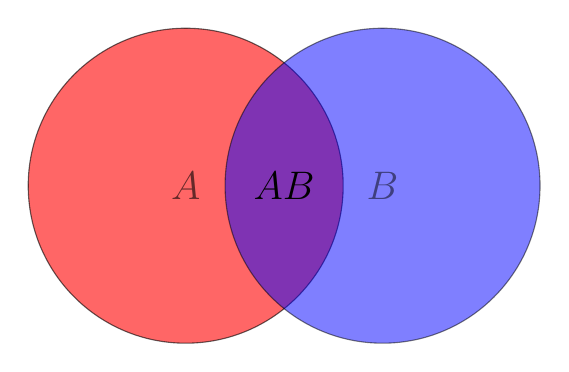
\begin{tikzpicture}
        \draw[fill=red,opacity=0.6] (0, 0) circle (2) node {\Large$A$};
        \draw[fill=blue,opacity=0.5] (2.5, 0) circle (2) node {\Large$B$};
        \node (A) at (1.25, 0) {\Large$A \intersection B$};
    \end{tikzpicture}
}

\chapter{Probability}
\label{ch:probability}

\section{Axioms of Probability}

\begin{defn}\proofbreak
    \begin{itemize}
        \item Sample point: a possible outcome of a probabilistic experiment, often denoted by $\omega$.
        \item Sample space: the set of all sample points, often denoted by $\Omega$.
        \item Event: any subset of the sample space.
    \end{itemize}
\end{defn}

\begin{defn}
    If events $A_i \subseteq \Omega$ are disjoint, we say that these events are \emph{mutually exclusive}.
\end{defn}

\begin{defn}\label{kolmogorov-probability-axioms}
    A \emph{probability space} is a sample space $\Omega$ together with a function $P: \mathcal{P}(\Omega) \to \R$ that satisfies the following axioms:
    \begin{itemize}
        \item Non-negativity: for any event $A \subseteq \Omega$, $P(A) \geq 0$.
        \item Normalization: $P(\Omega) = 1$.
        \item Countable-additivity: if $A_i$ are a countable sequence of mutually exclusive events, then \[P\left(\bigdisjointunion_{i}A_i\right) = \sum_{i}P(A_i).\]
    \end{itemize}
\end{defn}

\begin{rmk}
    These axioms are due to Andrey Kolmogorov.
\end{rmk}

\begin{prop}
    Let $(\Omega, P)$ be a probability space, and $A \subseteq \Omega$ an event. Then $P(A) + P(\complementof{A}) = 1$.
\end{prop}

\begin{proof}
    Since $A$ and $\complementof{A}$ are mutually exclusive, $P(A) + P(\complementof{A}) = P(A \union \complementof{A}) = P(\Omega) = 1$.
\end{proof}

\begin{cor}
    $P(\emptyset) = 0$.
\end{cor}

\begin{prop}Monotonicity\label{probability-monotonicity}\proofbreak
    Let $A, B \subseteq \Omega$ be events such that $A \subseteq B$. Then $P(A) \leq P(B)$.
\end{prop}

\begin{proof}
    Let $C = B - A$. Then $A \union C = B$ and $A \intersection C = \emptyset$. Since $A$ and $C$ are therefore mutually exclusive, $P(A) + P(C) = P(A \union C) = P(B)$. Since $P(C) \geq 0$ by the axiom of non-negativity, it follows that $P(A) \leq P(B)$.
\end{proof}

\begin{thm}{Inclusion-exclusion Principle}\label{inclusion-exclusion-probability}\proofbreak
    Let $A, B, C \subseteq \Omega$ be events. Then
    \[P(A \union B) = P(A) + P(B) - P(A \intersection B),\]
    and
    \begin{align*}
        P(A \union B \union C) &= P(A) + P(B) + P(C) \\
                               &- P(A \intersection B) - P((A \intersection C) - P(B \intersection C) \\
                               &+ P(A \intersection B \intersection C).
    \end{align*}
\end{thm}

\begin{proof}
    Since $A \union B = (A - B) \union (B - A) \union (A \intersection B)$, which are necessarily mutually exclusive events, we have
    \[P(A \union B) = P(A - B) + P(B - A) + P(A \intersection B).\]
    Now note that $A = (A - B) \union (A \intersection B)$ and $B = (B - A) \union (A \intersection B)$, and so $P(A) = P(A - B) + P(A \intersection B)$ and $P(B) = P(B - A) + P(A \intersection B)$. Therefore, \begin{align*}
        P(A \union B) &= P(A - B) + P(B - A) + P(A \intersection B) \\
                      &= \big[P(A - B) + P(A \intersection B)\big] + \big[P(B - A) + P(A \intersection B)\big] - P(A \intersection B) \\
                      &= P(A) + P(B) - P(A \intersection B).
    \end{align*}

    To prove the three-way version of the principle, we can apply the two-way version to $A \union B$ and $C$. This gives us
    \begin{align*}\label{inclusion-exclusion-three-intermediate}\tag{$1$}
        P(A \union B \union C) &= P(A \union B) + P(C) - P((A \union B) \intersection C) \\
        &= \big[P(A) + P(B) - P(A \intersection B)\big] + P(C) - P((A \union B) \intersection C).
    \end{align*}
    Since $(A \union B) \intersection C = (A \intersection C) \union (B \intersection C)$, we can apply the principle again to find that
    \[P((A \union B) \intersection C) = P(A \intersection C) + P(B \intersection C) - P((A \intersection C) \intersection (B \intersection C)).\] Noting that $(A \intersection C) \intersection (B \intersection C) = A \intersection B \intersection C$ and substituting this back into \ref{inclusion-exclusion-three-intermediate}, we obtain
    \begin{align*}
        P(A \union B \union C) &= P(A) + P(B) + P(C) - P(A \intersection B) - \big[P(A \intersection C) + P(B \intersection C) - P(A \intersection B \intersection )\big] \\
        &= P(A) + P(B) + P(C) \\
        &- P(A \intersection B) - P((A \intersection C) - P(B \intersection C) \\
        &+ P(A \intersection B \intersection C).
    \end{align*}
\end{proof}

\begin{prop}
    \[A \union B = A \disjointunion (B - A).\]
    \[A \union B \union C = A \disjointunion (B - A) \disjointunion (C - (A \union B)).\]
\end{prop}

\begin{prop}{Subadditivity}\label{subadditivity}\proofbreak
    Let $A_1, A_2, \ldots$ be a sequence of events. Then for any $n \geq 1$ we have
    \begin{align*}
        P\left(\bigunion_{i=1}^{n}A_i\right) \leq \sum_{i=1}^{n}P(A_i),\;\;\;\;
        P\left(\bigunion_{i=1}^{\infty}A_i\right) \leq \sum_{i=1}^{\infty}P(A_i).
    \end{align*}
\end{prop}

\begin{proof}
    Let $B_0 = \bigunion_{i=1}^{\infty}A_i$, and then form the sequence $B_1, B_2, \ldots$ defined by $B_i = A_i - B_0$. Note that this implies $P(B_i) \leq P(A_i)$. We know that the sequence $B_0, B_1, B_2, \ldots$ are mutually exclusive, and so
    \begin{align*}
        P\left(\bigdisjointunion_{i=0}^{\infty}B_i\right) = P(B_0) + \sum_{i=1}^{\infty}P(B_i) \leq \sum_{i=1}^{\infty}P(A_i).
    \end{align*}
    Since $\bigdisjointunion_{i=0}^{\infty}B_i = \bigunion_{i=1}^{\infty}A_i$, we then have
    \begin{align*}
        P\left(\bigdisjointunion_{i=1}^{\infty}A_i\right) \leq \sum_{i=1}^{\infty}P(A_i).
    \end{align*}
    The proof for a finite sequence is analogous.
\end{proof}

\begin{exmp}{Finite, equally-likely probability law}\proofbreak
    Let $(\Omega, P)$ be a sample space together with a function $P: \mathcal{P}(\Omega) \to \R$, where $\abs{\Omega} \in \Z^{+}$ and for all $A \in \mathcal{\Omega}$, \[P(A) = \frac{\abs{A}}{\abs{\Omega}}.\]

    Since $\abs{A} \geq 0$ and $\abs{\Omega} > 0$, $P(A) \geq 0$ and so this model satifies the non-negativity axiom. Since $P(\Omega) = \frac{\abs{\Omega}}{\abs{\Omega}} = 1$, this model satisfies the normalization axiom.
    
    Let $A = A_1 \disjointunion A_2 \disjointunion \cdots$. Then
    \begin{align*}
        P(A) = \frac{\abs{A_1 \disjointunion A_2 \disjointunion \cdots}}{\abs{\Omega}} = \frac{\abs{A_1}}{\abs{\Omega}} + \frac{\abs{A_2}}{\abs{\Omega}} + \cdots = P(A_1) + P(A_2) + \cdots,
    \end{align*}
    and so this model also satisfies the countable-additivity axiom. Therefore, it is a probability space.
\end{exmp}

\begin{exmp}{Discrete probability law}\proofbreak
    Let $\Omega$ be a sample space such that $\abs{\Omega}$ is countable, and let $M: \Omega \to R$ be a mass-function: $M(\omega) \geq 0$ for all $\omega \in \Omega$, and $\sum_{\omega \in \Omega}M(\omega) = 1$.

    Now consider $P: \mathcal{P}(\Omega) \to \R$ defined by
    \[P(A) = \sum_{\omega \in A}M(\omega).\]

    Since $M(\omega) \geq 0$, $P(A) \geq$ and so $P$ satisfies the axiom of non-negativity. Since \[P(\Omega) = \sum_{\omega \in \Omega}M(\omega) = 1\] by the definition of $M$, $P$ satisfies the axiom of normalization. Finally, for $A = A_1 \disjointunion A_2 \disjointunion \cdots$,
    \begin{align*}
        P(\bigdisjointunion_{i}A_i) = \sum_{i}P(A_i) = \sum_{i}\sum_{\omega \in A_i}M(\omega) = \sum_{\omega \in A}M(\Omega) = P(A).
    \end{align*}
    Therefore, $P$ satisfies the axiom of countable additivity and so $(\Omega, P)$ is a probability space.
\end{exmp}

\begin{exmp}{Geometric probability law}\proofbreak
    Let $\Omega = \{\omega_1, \omega_2, \ldots\}$ be a sample space such that $\abs{\Omega} = \abs{\Z}$, and define $P: \mathcal{P}(\Omega) \to \R$ by
    \[P(A) = \sum_{\omega_i \in A}\left(\frac{1}{2}\right)^{i}.\]
    
    Since $\left(\frac{1}{2}\right)^i \geq 0$, $P(A) \geq 0$ and so $P$ satisfies the axiom of non-negativity. Since
    \begin{align*}
        P(\Omega) = \sum_{\omega_i \in \Omega}\left(\frac{1}{2}\right)^{i} = \sum_{i=1}^{\infty}\left(\frac{1}{2}\right)^{i} = \frac{1/2}{1 - 1/2} = 1,
    \end{align*}
    we know that $P$ satisfies the axiom of normalization.

    Finally, for $A = A_1 \disjointunion A_2 \disjointunion \cdots$,
    \begin{align*}
        P\left(\bigdisjointunion_{i}A_i\right) = \sum_{\omega_j \in A}\left(\frac{1}{2}\right)^{j} = \sum_{i}\sum_{\omega_j \in A_i}\left(\frac{1}{2}\right)^{j} = \sum_{i}P(A_i).
    \end{align*}
    Therefore, $P$ satisfies the axiom of countable additivity and so $(\Omega, P)$ is a probability space.
\end{exmp}

\section{Conditional Probability}

\begin{exmp}
    Roll two six-sided dice, and only look at one of them. It is a six. Let $S$ denote the event that the sum of the values of the two dice is seven, and $A$ is the event that at least one of dice was a six. What is the probability of $P(S | A)?$ It is $\frac{2}{11}$, not $\frac{1}{6}$.
\end{exmp}

\begin{defn}
    Let $A, B \in \Omega$. Then the probability that $A$ occurred, given that $B$ occured, is denoted by $P(A | B)$ and read as ``the probability of $A$ given $B$''.
\end{defn}

\begin{prop}
    If all sample points in $\Omega$ are equally likely, then $P(A | B) = \frac{P(A \intersection B)}{P(B)}$.
\end{prop}

\begin{cor}
    $P(A \intersection B) = P(A | B)P(B)$.
\end{cor}

\begin{thm}
    Let $(\Omega, P)$ be a probability space, and $B \subseteq \Omega$ an event such that $P(B) > 0$. Then $(B, P(\cdot | B))$ form a probability space.
\end{thm}

\begin{proof}
    To show that $(B, P(\cdot|B))$ is a probability space, we need to show non-negativity (that $P(A | B) \geq 0$ for all $A$), normalization (that $P(B|B) = 1$), and countable additivity (that $P(A_1 \disjointunion A_2 \disjointunion \cdots | B) = P(A_1 | B) + P(A_2 | B) + \cdots$ if $A_i$ is a countable sequence).

    For any $A \subseteq B$, we know that $P(A \intersection B), P(B) \geq 0$, and so \[P(A | B) = \frac{P(A \intersection B)}{P(B)} \geq 0.\]

    \[P(B | B) = \frac{P(B \intersection B)}{P(B)} = \frac{P(B)}{P(B)} = 1.\]

    \begin{align*}
        P(A_1 \disjointunion A_2 \disjointunion \cdots | B) &= \frac{P\left((A_1 \disjointunion A_2 \disjointunion \cdots) \intersection B\right)}{P(B)} = \frac{P(A_1 \intersection B) \disjointunion (A_2 \intersection B) \disjointunion \cdots)}{P(B)} \\
        &= \frac{P(A_1 \intersection B) + P(A_2 \intersection B) + \cdots)}{P(B)} = \frac{P(A_1 \intersection B)}{P(B)} + \frac{P(A_2 \intersection B)}{P(B)} + \cdots \\
        &= P(A_1 | B) + P(A_2 | B) + \cdots.
    \end{align*}
\end{proof}

\begin{exmp}
    Consider a sequence of coin tosses. Let $B$ be the event that the first head of the sequence occurs on an odd numbered toss (the first toss is \#1), and let $A$ be the event that the event first coin toss lands on heads. What is $P(A | B)$?

    Since $A \subseteq B$, we know that $A \intersection B = A$. Furthermore, $P(A) = \frac{1}{2}$, and $P(B) = \frac{1}{2} + \frac{1}{8} + \cdots = \frac{1/2}{1-1/4} = \frac{1}{2}\cdot\frac{4}{3} = \frac{2}{3}$. Therefore, \[P(A | B) = \frac{P(A \intersection B)}{P(B)} = \frac{P(A)}{P(B)} = \frac{1}{2}\cdot\frac{3}{2} = \frac{3}{4}.\]
\end{exmp}

\begin{thm}Law of Total Probability\label{total-probability}\proofbreak
    Let $B_1, \ldots, B_n \in \Omega$ be mutually exclusive and exhaustive events. Then for any event $A \in \Omega$,
    \[P(A) = \sum_{i=1}^{n}P(A \intersection B_i) = \sum_{i=1}^{n}P(A | B_i)P(B_i).\]
\end{thm}

\begin{proof}
    Note that if $x \in (A \intersection B_i)$ and $x \in (A \intersection B_j)$, then $x \in B_i$ and $x \in B_j$. Since $B_1, \ldots, B_n$ are mutually exclusive they are disjoint, and so we must have $i = j$. Therefore, $A \intersection B_1, A \intersection B_2, \ldots, A \intersection B_n$ are disjoint.

    Also note that
    \begin{align*}
        \bigdisjointunion_{i=1}^{n}A \intersection B_i = A \intersection \left(\bigdisjointunion_{i=1}^{n}B_i\right) = A \intersection \Omega = A
    \end{align*}
    since $B_1, \ldots, B_n$ are exhaustive.

    Therefore, by the axiom of countable additivity,
    \begin{align*}
        P(A) = P\left(\bigdisjointunion_{i=1}^{n}A \intersection B_i\right) = \sum_{i=1}^{n}P(A \intersection B_i).
    \end{align*}
\end{proof}

\begin{exmp}
    Consider a box containing six coins. Three of these coins are fair, but one of them has two tails, and the remaining two have two heads each. If we randomly (uniformly) select one coin and flip it twice, what is the probability it comes up heads twice?

    Let $A$ be the event we observe two heads. Let $B_1$ be the event we selected one of the fair coins, $B_2$ the event we selected the $2$-tailed coin, and $B_3$ the event that we selected the $2$-headed coin. Then by the Law of Total Probability \ref{total-probability},
    \[P(A) = \sum_{i=1}^{n}P(A | B_i)P(B_i) = \left(\frac{1}{4}\cdot\frac{3}{6}\right) + \left(\frac{0}{1}\cdot\frac{1}{6}\right) + \left(\frac{1}{1}\cdot\frac{2}{6}\right) = \frac{1}{8} + \frac{1}{3} = \frac{11}{24}.\]
\end{exmp}

\begin{thm}{Bayes' Rule}\proofbreak
    Let $B_1, \ldots, B_n \in \Omega$ be mutually exclusive and exhaustive events. Then for any event $A \in \Omega$,
    \begin{align*}
        P(B_k | A) = \frac{P(A|B_k))P(B_k)}{\sum_{k}P(A \intersection B_k)} = \frac{P(A|B_k))P(B_k)}{\sum_{k}P(A | B_k)P(B_k)}.
    \end{align*}
\end{thm}

\section{Independence}

\begin{defn}
    Events $A, B \in \Omega$ are \emph{independent} if $P(A \intersection B) = P(A)P(B)$.
\end{defn}

\begin{prop}
    If $A$ and $B$ are independent events, then $P(A | B) = P(A)$ and $P(B | A) = P(B)$.
\end{prop}

\begin{proof}
    \[P(A | B) = \frac{P(A \intersection B)}{P(B)} = \frac{P(A)P(B)}{P(B)} = P(A)\]
\end{proof}

\begin{prop}
    If $A$ and $B$ are independent events, then $A$ and $\complementof{B}$ are independent.
\end{prop}

\begin{proof} Since $B$ and $\complementof{B}$ are necessarily mutually exclusive and exhaust $A$, we have $A = (A \intersection B) \disjointunion (A \intersection \complementof{B})$. Furthermore, $P(\complementof{B}) = 1- P(B)$. Then
    \begin{align}
        P(A \intersection \complementof{B}) &+ P(A \intersection B) = P(A) \\
        P(A \intersection \complementof{B}) &+ P(A)P(B) = P(A) \\
        P(A \intersection \complementof{B}) &= P(A)\left(1 - P(B)\right).
    \end{align}
\end{proof}

\begin{defn}
    We say events $A_1, A_2, \ldots$ are \emph{independent} if every for every finite subcollection $A_{i_1}, A_{i_2}, \ldots, A_{i_k}$ we have
    \[P(A_{i_1} \intersection A_{i_2} \intersection \cdots \intersection A_{i_k}) = P(A_{i_1})P(A_{i_2})\cdots P(A_{i_k}).\]
\end{defn}

\section{Random Variables}

\begin{defn}
    A \emph{random variable} $X$ on a sample space $\Omega$ is a function $X: \Omega \to \R$.
\end{defn}

\begin{exmp}
    Let $A \subseteq \Omega$ be an event, and let
    \[X: \omega \mapsto \begin{dcases}
        1, & \omega \in A \\
        0, & \omega \not\in A
    \end{dcases}.\]
    Then $X$ is a random variable.
\end{exmp}

\begin{defn}
    A random variable $X$ is said to be a \emph{discrete} random variable when its image $X(\Omega)$ is countable.
\end{defn}

\begin{defn}
    The \emph{Bernoulli distribution} is the probability distribution of a random variable that takes value $1$ with probability $0 \leq p \leq 1$, and value $0$ with probability $1 - p$. For a random variable $X$ with this distribution and $k \in \{0, 1\}$:
    \[P(X = k) = \begin{dcases}
        p, & k = 1  \\
        1 - p, & k = 0
    \end{dcases} = p^k(1-p)^{1-k}.\]
\end{defn}

\begin{defn}
    The \emph{binomial} distribution with parameters $n$ and $p$ is the distribution of the number of successes in a sequence of $n$ independent trials which can take values $1, 0$ with probability $p$ and $1 - p$. The probability of $ 0 \leq k \leq n$ successes is
    \[P(X = k) = \binom{n}{k}p^k(1 - p)^{n-k}.\]
\end{defn}

\begin{defn}
    The \emph{Poisson} distribution with parameter $\lambda > 0$, is the distribution of the number of independent events that occur in a fixed period when the events occur at a constant rate with $\lambda$ events per period on average. The probability of $k$ events during this period is
    \[P(X = k) = \frac{e^{-\lambda}\lambda^k}{k!}.\]
    Alternatively, if the independent events occur at a rate of $r$ per unit period, in a period of length $t$, we can use $\lambda = rt$.
\end{defn}

\begin{defn}
    The \emph{geometric} distribution with parameter $0 \leq p \leq 1$ is the distribution of the number of independent Bernoulli $p$ trials needed to get the first success. It is given by
    \[P(X = k) = (1-p)^{k-1}p.\]
\end{defn}

\begin{defn}
    The \emph{negative binomial distribution} is a generalization of the geometric distribution. Rather than the distribution of the first success in a series of independent Bernoulli $p$ trials, it is the distribution of the $r$th success in such a series. For $k \geq r$, it is given by
    \[P(X = k) = \binom{k-1}{r-1}p^r(1-p)^{k-r}.\]
\end{defn}

\begin{defn}
    The \emph{expected value} of a discrete random variable $X$ with probability mass function $P(X)$ is
    \[E(X) = \sum_{x \in \Omega}xP(X = x).\]
\end{defn}

\begin{exmp}
    Consider a discrete random variable $X$ with a Bernoulli $p$ distribution. The expected value of $X$ is
    \begin{align*}
        E(X) = \sum_{x \in {0, 1}}xP(X = x) = 0(1-p) + 1(p) = p.
    \end{align*}
\end{exmp}

\begin{exmp}
    Consider a discrete random variable $X$ with a binomial $n, p$ distribution. The expected value of $X$ is then
    \begin{align*}
        E(X) &= \sum_{x \in {0, 1, \ldots, n}}xP(X = x) \\
             &= \sum_{x=1}^{n}x\binom{n}{x}p^x(1 - p)^{n-x} \\
             &= \sum_{x=1}^{n}x\frac{n!}{x!(n-x)!}p^x(1 - p)^{n-x} \\
             &= p\sum_{x=1}^{n}\frac{n!}{(x-1)!(n-x)!}p^{x-1}(1 - p)^{n-x} \\
             &= np\sum_{x=0}^{n-1}\frac{(n-1)!}{x!(n-x-1)!}p^x(1 - p)^{n-x-1} \\
             &= np\sum_{x=0}^{n-1}\binom{n-1}{x}p^x(1 - p)^{(n-1)-x} \\
             &= np\left(p+(1-p)\right)^{n-1} = np.
    \end{align*}
\end{exmp}

\begin{prop}
    Expectation is linear, that is $E(kX_1+X_2) = kE(X_1) + E(X_2)$.
\end{prop}

\begin{proof}
    Follows from linearity of sums.
\end{proof}

\begin{thm}{Law of the Unconscious Statistician ($\mathcal{LOTUS}$)}{\label{lotus}}\proofbreak
    Let $X$ be a discrete random variable with expected value $E(X)$. For any function $f$, \[E[f(X)] = \sum_{x}f(x)P(X=x).\]
\end{thm}

\begin{defn}
    Let $X$ be a discrete random variable. For $k \geq 1$, the $k$th \emph{moment} of $X$ is the expected value of $X^k$.
\end{defn}

\begin{rmk}
    The mean of a random variable $X$ (denoted by $\mu$) is the first moment of $X$.
\end{rmk}

\begin{exmp}
    All moments of a Bernoulli $p$ distribution are simply $p$.
\end{exmp}

\begin{defn}
    For a random variable $X$, the \emph{variance} of $X$ is the expected squared distance from the mean: \[\varianceof{X} = E\left[\left(X-E(X)\right)^2\right] = E\left[\left(x - \mu\right)^2\right].\]
\end{defn}

\begin{rmk}
    While the mean has the same units as $X$, the variance has measure of those units squared.
\end{rmk}

\begin{defn}
    The \emph{standard deviation} $\sigma$ of a random variable $X$ is the positive square root of the variance of $X$.
\end{defn}

\begin{prop}
    When the first and second moments of a random variable exist and are finite, the variance can be computed by $\sigma^2 = E(X^2) - E(X)^2$.
\end{prop}

\begin{proof}
    By $\mathcal{LOTUS}$ \ref{lotus}, the variance is
    \begin{align*}
        E\left[(X-E(X))^2\right] &= E\left[X^2 - 2XE(X) + E(X)^2\right] \\
        &= E(X^2) - 2E(X)E\left[X\right] + E\left[E(X)^2\right] \\
        &= E(X^2) - 2E(X)^2 + E(X)^2 = E(X^2) - E(X)^2.
    \end{align*}
\end{proof}

\begin{exmp}
    Let $X$ be a binomial $n, p$ distribution. Recall that the mean of $X$ is $np$. Note that $E(X^2) = E[X(X-1)+X]$, and by $\mathcal{LOTUS}$ \ref{lotus}
    \begin{align*}
        E(X(X-1)) &= \sum_{x=0}^{n}x(x-1)\frac{n!}{x!(n-x)!}p^x(1-p)^{n-x} \\
        &= \sum_{x=2}^{n}\frac{n!}{(x-2)!(n-x)!}p^x(1-p)^{n-x} \\
        &= n(n-1)p^2\sum_{x=2}^{n}\frac{(n-2)!}{(x-2)!(n-x)!}p^{(x-2)}(1-p)^{n-x} \\
        &= n(n-1)\sum_{x=0}^{n-2}\frac{(n-2)!}{x!((n-2)-x)!}p^x(1-p)^{(n-2)-x} \\
        &= n(n-1)p^2\left(p+(1-p)\right)^{n-2} = n(n-1)p^2.
    \end{align*}
    Therefore, $E(X^2) = E[X(X-1)]+E[X]=n(n-1)p^2+np = n^2p^2+np-np^2$, and so the variance is $E(X^2)-E(X)^2 = n^2p^2+np-np^2-n^2p^2 = np-np^2 = n(p-p^2)$.
\end{exmp}

\begin{defn}
    Given a random variable $X$, the \emph{moment generating function} for $\theta \in \R$ is
    \begin{align*}
        M(\theta) = E(e^{\theta X}).
    \end{align*}
\end{defn}

\begin{prop}
    If the moment generating function exists for a particular random variable,
    \begin{enumerate}
        \item it uniquely identifies that random variablem i.e. it is injective,
        \item all moments of the random variable exist and are finite,
        \item the $n$th derivative of the moment generating function at $\theta = 0$ is the $n$th moment of the random variable.
    \end{enumerate}
\end{prop}

\begin{prop}\proofbreak
    3) Consider the Maclaurin series of $e^{\theta X}$, which is
    \[e^{\theta X} = \sum_{n=0}^{\infty}\frac{(\theta X)^n}{n!} = 1 + X\theta + X^2\frac{\theta^2}{2} + \cdots.\]
    Then by linearity of the expected value and by linearity of the derivative, $M^{(k)}(0) = E\left[X^k\right]$.
\end{prop}

\begin{exmp}
    Consider the Poisson $\mu$ distribution, where $P(X = x) = \frac{e^{-\mu}\mu^x}{x!}$. The moment generating function, if it exists, by $\mathcal{LOTUS}$ \ref{lotus} would be given by
    \begin{align*}
       E(e^{\theta X})] &= \sum_{x=0}^{\infty}e^{\theta x}P(X = x) \\
       &= \sum_{x=0}^{\infty}e^{\theta x}\frac{e^{-\mu}\mu^x}{x!} \\
       &= e^{-\mu}\sum_{x=0}^{\infty}\frac{\left(\mu e^{\theta}\right)^{x}}{x!} \\
       &= e^{-\mu}e^{e^{\theta}\mu} = e^{\mu(e^{\theta-1})}.
    \end{align*}
\end{exmp}

\section{Cumulative Distribution Functions}

\begin{defn}
    Given a random variable $X$, the function $p(x) = P(X = x)$ is the \emph{probability mass function} (or PMF) of $X$.
\end{defn}

\begin{defn}
    Given a random variable $X$, the function $F: \R \to [0, 1]$ defined by
    \[x \mapsto P(X \leq x)\]
    is the \emph{cumulative distribution function} (or CDF) of $X$.
\end{defn}

\begin{prop}
    Given a random variable $X$ with CDF $F_X$, for any $x < y$, then $F_X(x) \leq F_X(y)$.
\end{prop}

\begin{proof}
    If $x < y$ then the event $X \leq x$ is a subset of the event $X \leq y$, so $P(X \leq x) \leq P(X \leq y)$ by Proposition \ref{probability-monotonicity}.
\end{proof}

\begin{thm}{Continuity of Probability}\label{continuity-of-probability}\proofbreak
    Consider sequences of events $E_i \in \Omega$ such that
    \begin{align*}
        E_1 \subseteq E_2 \subseteq E_3 \subseteq \cdots,
    \end{align*}
    or
    \begin{align*}
        E_1 \supseteq E_2 \supseteq E_3 \supseteq \cdots.
    \end{align*}

    Then
    \begin{align*}
        \lim_{n \to \infty}P(E_n) = P\left(\lim_{n \to \infty}E_n\right).
    \end{align*}
\end{thm}

\begin{proof}
    Consider the case of increasing events, so $E_1 \subseteq E_2 \cdots$. Let $F_n = E_n - \union_{i < n}E_i$. Then
    \begin{align*}
        \bigcup_{i=1}^{n}E_i = \bigsqcup_{i=1}^{n}F_i,\;\;\;\bigcup_{i=1}^{\infty}E_i = \bigsqcup_{i=1}^{\infty}F_i.
    \end{align*}
    Therefore,
    \begin{align*}
        P\left(\lim_{n \to \infty} E_n\right) &= P\left(\bigcup_{i=1}^{\infty}E_i\right) = P\left(\bigcup_{i=1}^{\infty}F_i\right) = \sum_{i =1}^{\infty}P(F_i) \\
        &= \lim_{n \to \infty}\sum_{i}^{n}P(F_i) = \lim_{n \to \infty} P\left(\bigsqcup_{i}^{n}F_i\right) = \lim_{n \to \infty} P\left(\bigcup_{i}^{n}E_i\right) = \lim_{n \to \infty}P(E_n).
    \end{align*}

    Now consider the case where $E_1 \supseteq E_2 \cdots$. Notice that $\complementof{E_1} \subseteq \complementof{E_2} \cdots$, so $\complementof{E_i}$ forms an increasing sequence of events. Therefore,
    \begin{align*}
        \lim_{n \to \infty}P(\complementof{E_n}) = P\left(\lim_{n \to \infty}\complementof{E_n}\right) = P\left(\bigcup_{i}^{\infty}\complementof{E_i}\right).
    \end{align*}
    Since
    \begin{align*}
        \bigcup_{i}^{\infty}\complementof{E_i} = \complementof{\left(\bigcap_{i}^{\infty}E_i\right)},
    \end{align*}
    it follows that
    \begin{align*}
        \lim_{n \to \infty}P(\complementof{E_n}) = P\left(\complementof{\left(\bigcap_{i}^{\infty}E_i\right)}\right) = 1 - P\left(\bigcap_{i}^{\infty}E_i\right).
    \end{align*}
    Since $1 - P(E_i) = P(\complementof{E_i})$, we then have
    \begin{align*}
        \lim_{n \to \infty}P(\complementof{E_n}) = \lim_{n \to \infty}\left(1 - P(E_n)\right) = 1 - \left(\lim_{n \to \infty}P(E_n)\right).
    \end{align*}
    It follows that
    \begin{align*}
        \lim_{n \to \infty}P(E_n) = P\left(\bigcap_{i}^{\infty}E_i\right) = P\left(\lim_{n \to \infty}E_n\right).
    \end{align*}
\end{proof}

\begin{prop}
    Given a random variable $X$ with CDF $F$, $F$ is right-continuous for all $x \in \R$:
    \[\forall x \in \R,\;\;\lim_{n \to\infty}F(x + \frac{1}{n}) = F(x),\]
    and left-limits exist for all $x \in \R$:
    \[\forall x \in \R,\;\;\lim_{n \to \infty}F(x - \frac{1}{n}).\]
\end{prop}

\begin{proof}
    The event that $X \leq x$ is
    \begin{align*}
        \bigcap_{n = 1}^{\infty}(X \leq x + \frac{1}{n}),
    \end{align*}
    and so by the continuity of probability \ref{continuity-of-probability} right-continuity follows:
    \begin{align*}
        F(x) = P(X \leq x) = \lim_{n \to \infty}P(X \leq x + \frac{1}{n}) = \lim_{n \to \infty}F(x + \frac{1}{n}).
    \end{align*}

    Similarly,
    \begin{align*}
        \lim_{n \to \infty}F(x - \frac{1}{n}) = \lim_{n \to \infty}P(X \leq x - \frac{1}{n}) = P(X < x),
    \end{align*}
    so the left limits always exist. Note that $P(X < x)$ will not equal $P(X \leq x)$ if $P(X = x) > 0$, so $F$ may not be left-continuous.
\end{proof}

\begin{defn}
    A random variable with a continuous CDF is a \emph{continuous} random variable.
\end{defn}

\begin{prop}
    Given a continuous random variable $X$, $P(X = x) = 0$ for all $x$.
\end{prop}

\begin{proof}
    Let $F_X(x) = P(X \leq x)$ be the (continuous) CDF of $X$. Fix some $x$. Then for any $h > 0$,
    \begin{align*}
        P(x-h < X \leq x) = F(x) - F(x - h).
    \end{align*}
    Therefore, as $h \to 0$, $P(x - h < X \leq x) \to 0$. Therefore, $P(x < X \leq x) = 0$, and so $P(X = x) = 0$.
\end{proof}

\begin{defn}
    The \emph{probability density function} (PDF) of a continuous random variable $X$ is
    \begin{align*}
        f(x) = \lim_{h \to 0}\frac{P(x - h < X \leq x)}{h} = \lim_{h \to 0}\frac{F(x) - F(x-h)}{h}.
    \end{align*}
\end{defn}

\begin{rmk}
    Not all continuous random variables possess a PDF, since the limit may not exist. Every continuous CDF can be decomposed into a linear combination of two functions: a \emph{absolutely continuous} part and a \emph{singlular continuous} part. The Cantor function is an example of a CDF whose absolutely continuous part is zero.
\end{rmk}

\begin{thm}
    Let $F(x)$ be the CDF and $f(x)$ the PDF of an absolutely continuous random variable $X$. Then:
    \begin{enumerate}
        \item $F'(x) = f(x)$,
        \item $F(x) = \int_{-\infty}^{x}f(x)dx$,
        \item $f(x)$ exists almost everywhere,
        \item $\int_{-\infty}^{\infty}f(x)dx = 1$.
    \end{enumerate}
\end{thm}

\begin{proof}\proofbreak
    \begin{enumerate}
        \item Definition of $f(x)$,
        \item Follows from above,
        \item Follows from absolute continuity of $F(x)$,
        \item Follows from absolute continuity of $F(x)$.
    \end{enumerate}
\end{proof}

\begin{cor}
    \begin{align*}
        P(a < X \leq b) &= P(X \leq b) - P(X \leq a) \\
        &= F(b) - F(a) \\
        &= \int_{-\infty}^{b}f(x)dx - \int_{-\infty}^{a}f(x)dx \\
        &= \int_{a}^{b}f(x)dx.
    \end{align*}
\end{cor}

\begin{prop}
    A function $f: \R \to \R$ is a probability density function when $f(x) \geq 0$, $f(x)$ is defined for all $\R$, and $\int_{-\infty}^{\infty}f(x)dx = 1$.
\end{prop}

\begin{defn}
    A random variable $X$ has the \emph{exponential} distribution with parameter $\lambda > 0$ when its probability density function is
    \begin{align}
        f(x) = \begin{dcases}
            \lambda e^{-\lambda x}, & x > 0 \\
            0, & x \leq 0
        \end{dcases}.
    \end{align}
\end{defn}

\begin{exmp}
    This is a probability density function since $f(x)$ is clearly non-negative, defined for all $x \in \R$, and
    \begin{align*}
        \int_{-\infty}^{\infty}f(x)dx &= \int_{0}^{\infty}f(x)dx = \int_{0}^{\infty}\lambda e^{-\lambda x}dx \\
        &= \lambda \frac{1}{-\lambda}e^{-\lambda x}\big\rvert_{0}^{\infty} = 0 - (-e^{0}) = 1.
    \end{align*}
\end{exmp}

\begin{defn}
    The expected value of a continuous random variable $X$ with probability density function $f_X(x)$ is
    \begin{align*}
        E(X) = \int_{-\infty}^{\infty}xf_X(x)dx.
    \end{align*}
\end{defn}

\begin{exmp}
    The expected value of a random variable $X \distributed \mathrm{exp}(\lambda)$ is
    \begin{align*}
        E(X) = \int_{-\infty}^{\infty}xf_X(x)dx = \int_{0}^{\infty}x\lambda e^{-\lambda x}dx.
    \end{align*}
    Integrating by parts, we let $u = x$ and $dv = \lambda e^{-\lambda x}dx$. Therefore, $du = dx$ and $v = -e^{-\lambda x}$. It follows that
    \begin{align*}
        \int x\lambda e^{-\lambda x}dx &= \int udv = uv - \int vdu = -xe^{-\lambda x} + \int e^{-\lambda x}dx \\
        &= -xe^{-\lambda x} - \frac{1}{\lambda}e^{-\lambda x} = -e^{-\lambda x}\left(x + \frac{1}{\lambda}\right).
    \end{align*}

    Note that since $\lambda > 0$, by L'Hopital's rule we have
    \begin{align*}
        \lim_{x \to \infty}xe^{-\lambda x} = \lim_{x \to \infty}\frac{x}{e^{\lambda x}} = \lim_{x \to \infty}\frac{1}{\lambda e^{\lambda x}} = 0.
    \end{align*}

    Therefore,
    \begin{align*}
        E(X) = \left(-e^{-\lambda x}\left(x + \frac{1}{\lambda}\right)\right)\big\rvert_{0}^{\infty} = 0 - \left(-\left(0 + \frac{1}{\lambda}\right)\right) = \frac{1}{\lambda}.
    \end{align*}

    The second moment of $X$ is
    \begin{align*}
        E(X^2) = \int_{-\infty}^{\infty}x^2f_X(x)dx = \int_{0}^{\infty}x\lambda e^{-\lambda x}dx.
    \end{align*}
    We can apply integration by parts twice to obtain $E(X^2)$
\end{exmp}

\begin{defn}
    A random variable $X$ has the \emph{uniform} distribution with parameters $a, b$ ($a < b$) when its probability density function is
    \begin{align}
        f(x) = \begin{dcases}
            0, & x \leq a \\
            \frac{1}{b - a}, & a < x < b \\
            0, & x \geq b
        \end{dcases}.
    \end{align}
\end{defn}

\begin{defn}
    The first moment (expected value) of a random variable $X \distributed \mathrm{uniform}(a, b)$ is
    \begin{align*}
        E(X) = \int_{-\infty}^{\infty}xf_X(x)dx = \int_{a}^{b}\frac{x}{b - a}dx = \frac{1}{b - a}\int_{a}^{b}xdx = \frac{b^2 - a^2}{2(b - a)} = \frac{(b - a)(b + a)}{2(b - a)} = \frac{b+a}{2}.
    \end{align*}

    The second moment is
    \begin{align*}
        E(X^2) = \int_{-\infty}^{\infty}x^2f_X(x)dx = \int_{a}^{b}\frac{x^2}{b - a}dx = \frac{b^3 - a^3}{3(b - a)} = \frac{(b-a)(b^2 + ab + a^2)}{3(b - a)} = \frac{b^2+ab+a^2}{3}.
    \end{align*}

    Therefore, the variance is
    \begin{align*}
        \sigma^2 = E(X^2) - E(X)^2 = \frac{b^2+ab+a^2}{3} - \left(\frac{b+a}{2}\right)^2 = \frac{b^2-2ab+a^2}{12}.
    \end{align*}
\end{defn}

\begin{rmk}
    When higher moments of random variables exist, there are additional quantities we can consider to understand distributions.
\end{rmk}

\begin{defn}
    The \emph{skewness} of a random variable $X$ is
    \begin{align*}
        E\left[\left(\frac{X-\mu}{\sigma}\right)^3\right]
    \end{align*}
\end{defn}

\begin{defn}
    The \emph{kurtosis} of a random variable $X$ is
    \begin{align*}
        E\left[\left(\frac{X-\mu}{\sigma}\right)^4\right]
    \end{align*}
\end{defn}

\begin{rmk}
    Skewness quantifies how skewed the distribution is --- positive skewness means it is right-tailed, and negative skewness means it is left tailed. When the skewness is zero, the distribution is perfectly symmetrical around its mean.

    Kurtosis measure how heavy the tails of the distribution are.
\end{rmk}

\begin{rmk}
    From the moment generating function, we can show that the $k$th moment of an exponentially distributed random variable is $k!\lambda^{-k}$. From there, we can calculate that the skewness of the exponential distribution is $2$ and the kurtosis is $9$, regardless of the specific value of $\lambda$.
\end{rmk}

\section{Gamma Distribution}

\begin{defn}
    The Euler gamma function is
    \begin{align*}
        \Gamma(\alpha) = \int_{0}^{\infty}x^{\alpha-1}e^{-x}dx.
    \end{align*}
    for $\alpha \in \C$ where $\alpha \neq 0$ and $\alpha$ is not a negative even integer.
\end{defn}

\begin{exmp}
    \begin{align*}
        \Gamma(1) = \int_{0}^{\infty}x^{1 - 1}e^{-x}dx = \int_{0}^{\infty}e^{-x}dx \\
        &= -e^{-x}\big\rvert_{0}^{\infty} = 1.
    \end{align*}
\end{exmp}

\begin{exmp}
    \begin{align*}
        \Gamma\left(\frac{1}{2}\right) = \int_{0}^{\infty}x^{-1/2}e^{-x}dx
    \end{align*}
    Let $x = u^2$, $dx = 2udu$. Then
    \begin{align*}
        \int_{0}^{\infty}\frac{1}{u}e^{-u^2}2udu = 2\int_{0}^{\infty}e^{-u^2}du.
    \end{align*}
    Then
    \begin{align*}
        \left(\Gamma\left(\frac{1}{2}\right)^2\right) = 4\int_{0}^{\infty}\int_{0}^{\infty}e^{-u^2}e^{-v^2}dudv.
    \end{align*}
    With a change to polar coordinates we obtain
    \begin{align*}
        \left(\Gamma\left(\frac{1}{2}\right)^2\right) = 4\int_{0}^{\pi/2}\int_{0}^{\infty}e^{-r^2}rdrd\theta = 4\int_{0}^{\pi/2}\frac{1}{2}d\theta = \pi.
    \end{align*}
    Therefore, $\Gamma(\frac{1}{2}) = \sqrt{\pi}$ since it is clear that $\Gamma(\frac{1}{2}) \geq 0$.
\end{exmp}

\begin{prop}
    For real $\alpha > 1$,
    \begin{align*}
        \Gamma(\alpha) = (\alpha - 1)\Gamma(\alpha - 1).
    \end{align*}
\end{prop}

\begin{proof}
    \begin{align*}
        \Gamma(\alpha) = \int_{0}^{\infty}x^{\alpha - 1}e^{-x}du.
    \end{align*}
    We can integrate this by parts to obtain
    \begin{align*}
        \Gamma(\alpha) = (\alpha - 1)\int_{0}^{\infty}x^{\alpha - 1 - 1}e^{-x}du.
    \end{align*}
    Therefore,
    \begin{align*}
        \Gamma(\alpha) = (\alpha - 1)\Gamma(\alpha - 1).
    \end{align*}
\end{proof}

\begin{rmk}
    $\Gamma(n+1) = n!$ for $n \in \Z$, $n \geq 0$, since $\Gamma(1) = 1$ and $\Gamma(n+1) = (n)(n-1)\cdots(3)(2)\Gamma(1)$.

    Additionally, if we know $\Gamma(x)$ for some $x \in (0, 1]$, then $\Gamma(x + n) = (x + n)(x + n - 1)\cdots(x + 1)\Gamma(x)$ for any $n \geq 0$.
\end{rmk}

\begin{prop}
    Let $f: \R \to \R_{\geq 0}$ have a finite integral. Then
    \begin{align*}
        g(x) = \frac{f(x)}{\int_{-\infty}^{\infty}f(x)dx}
    \end{align*}
    is a probability density function. This method of converting functions into a probability density function is called \emph{normalization}.
\end{prop}

\begin{exmp}
    Consider
    \begin{align*}
        g(x) = x^{a-1}e^{-x/\beta}
    \end{align*}
    for $x > 0$, and $g(x) = 0$ elsewhere for any $\alpha, \beta > 0$.

    With the substitution $u = x/\beta$,
    \begin{align*}
        \int_{-\infty}^{\infty}g(x)dx = \int_{0}^{\infty}(\beta u)^{\alpha -1}e^{-u}\beta du = \beta^{\alpha}\Gamma(\alpha).
    \end{align*}

    We can then normalize $g(x)$ to obtain the probability density function
    \begin{align*}
        f(x) = \begin{dcases}
            \frac{x^{a-1}e^{-x/\beta}}{\beta^{\alpha}\Gamma(\alpha)}, & x > 0 \\
            0, & x \leq 0
        \end{dcases}.
    \end{align*}

    This defines the Gamma$(\alpha, \beta)$ distribution, where $\alpha$ is the \emph{shape} parameter and $\beta$ is the \emph{scale} parameter.
\end{exmp}

\begin{rmk}
    The fact that the Gamma distribution's PDF integrates to $1$ can be used to solve other integrals. For example, consider.
    \begin{align*}
        \int_{0}^{\infty}x^{1/2}e^{-2x}dx.
    \end{align*}
    Let $f(x)$ be the PDF of the Gamma$(3/2, 1/2)$ distribution. Then
    \begin{align*}
        \int_{0}^{\infty}x^{1/2}e^{-2x}dx &= (1/2)^{3/2}\Gamma(3/2)\int_{0}^{\infty}\frac{x^{1/2}e^{-2x}}{(1/2)^{3/2}\Gamma(3/2)}dx = (1/2)^{3/2}\Gamma(3/2)\int_{0}^{\infty}f(x)dx \\
        &= \sqrt{\frac{1}{8}} \cdot \frac{1}{2}\Gamma\left(\frac{1}{2}\right) \cdot 1 = \frac{\sqrt{\pi}}{4\sqrt{2}}.
    \end{align*}
\end{rmk}

\begin{rmk}
    When $\alpha = 1$, the Gamma$(\alpha, \beta)$ distribution becomes the exp$\left(\frac{1}{\beta}\right)$ distribution.
\end{rmk}

\begin{prop}
    The mean of $X \distributed \mathrm{Gamma}(\alpha, \beta)$ is $\alpha\beta$.
\end{prop}

\begin{proof}
    \begin{align*}
        E(X) &= \int_{-\infty}^{\infty}xf_X(x)dx = \int_{0}^{\infty}x\left(\frac{x^{\alpha-1}e^{-x/\beta}}{\beta^{\alpha}\Gamma(\alpha)}\right)dx = \frac{1}{\beta^{\alpha}\Gamma(\alpha)}\int_{0}^{\infty}x^{\alpha}e^{-x/\beta}dx \\
        &= \frac{1}{\beta^{\alpha}\Gamma(\alpha)}\int_{0}^{\infty}x^{\alpha}e^{-x/\beta}dx = \frac{\beta^{\alpha+1}\Gamma(\alpha+1)}{\beta^{\alpha}\Gamma(\alpha)} = \beta\alpha.
    \end{align*}
\end{proof}

\begin{prop}
    The variance of $X \distributed \mathrm{Gamma}(\alpha, \beta)$ is $\alpha \beta^2$.
\end{prop}

\begin{proof}
    \begin{align*}
        E(X^2) &= \int_{-\infty}^{\infty}x^2f_X(x)dx = \int_{0}^{\infty}x^2\left(\frac{x^{\alpha-1}e^{-x/\beta}}{\beta^{\alpha}\Gamma(\alpha)}\right)dx = \frac{1}{\beta^{\alpha}\Gamma(\alpha)}\int_{0}^{\infty}x^{\alpha+1}e^{-x/\beta}dx \\
        &= \frac{1}{\beta^{\alpha}\Gamma(\alpha)}\int_{0}^{\infty}x^{\alpha+1}e^{-x/\beta}dx = \frac{\beta^{\alpha+2}\Gamma(\alpha+2)}{\beta^{\alpha}\Gamma(\alpha)} = \beta^2(\alpha+1)\alpha.
    \end{align*}

    The variance of $X \distributed \mathrm{Gamma}(\alpha, \beta)$ is therefore
    \begin{align*}
        E(X^2) - E(X)^2 = \beta^2(\alpha+1)\alpha - \alpha^2\beta^2 = \alpha\beta^2.
    \end{align*}
\end{proof}

\begin{prop}
    The moment generating function of $X \distributed \mathrm{Gamma}(\alpha, \beta)$ is
    \begin{align*}
        \left(1 - \beta\theta\right)^{-\alpha}.
    \end{align*}
\end{prop}

\begin{proof}
    \begin{align*}
        M(\theta) &= E(e^{\theta X}) = \int_{0}^{\infty}e^{\theta x}\frac{x^{\alpha-1}e^{-x/\beta}}{\beta^{\alpha}\Gamma(\alpha)}dx \\
        &= \frac{1}{\beta^{\alpha}\Gamma(\alpha)}\int_{0}^{\infty}x^{\alpha-1}e^{-x(1/\beta-\theta)}dx = \frac{\left[\left(\frac{1}{\beta}-\theta\right)^{-1}\right]^{\alpha}}{\beta^{\alpha}} = (1 - \beta\theta)^{-\alpha}.
    \end{align*}
\end{proof}

\section{Normal Distribution}

\begin{defn}
    A continuous random variable $X$ with the \emph{Normal} (or \emph{Gaussian}) distribution with parameters $\mu, \sigma$ has the probability density function
    \begin{align*}
        f(x) = \frac{e^{-\frac{1}{2}\left(\frac{x - \mu}{\sigma}\right)^2}}{\sigma\sqrt{2\pi}} = \frac{e^{-\frac{\left(x - \mu\right)^2}{2\sigma^2}}}{\sqrt{2\pi\sigma^2}}.
    \end{align*}
    We write $X \distributed \mathrm{Normal}(\mu, \sigma^2)$.
\end{defn}

\begin{defn}
    The \emph{standard normal distribution} is the normal distribution with $\mu = 0$ and $\sigma = 1$, and has probability density function
    \begin{align*}
        \varphi(x) = \frac{e^{-\frac{x^2}{2}}}{\sqrt{2\pi}}.
    \end{align*}
\end{defn}

\begin{rmk}\proofbreak
    \begin{itemize}
        \item For large $n$ and fixed $p$, the binomial$(n, p)$ distribution approximates the Normal distribution.
        \item For large $\lambda$, the Poisson distribution approximates the Normal distribution.
        \item For large $\alpha$ and fixed $\beta$, the Gamma distribution approximates the Normal distribution.
    \end{itemize}
\end{rmk}

\begin{thm}
    If $X \distributed \mathrm{Normal}(\mu, \sigma^2)$ and $Y = \alpha X + \beta$ where $\alpha \neq 0$, then
    \begin{align*}
        Y \distributed \mathrm{Normal}(\alpha\mu + \beta, \alpha^2\sigma^2).
    \end{align*}
\end{thm}

\begin{proof}
    Assume $\alpha > 0$. Then the CDF of $Y$ is $F_Y(y) = P(Y \leq y)$, which is $P(\alpha X + \beta \leq y)$ and so
    \begin{align*}
        F_Y(y) = P\left(X \leq \frac{y - \beta}{\alpha}\right) = \int_{-\infty}^{\frac{y-\beta}{\alpha}}\frac{e^{-\frac{1}{2}\left(\frac{x - \mu}{\sigma}\right)^2}}{\sqrt{2\pi\sigma^2}}dx.
    \end{align*}
    Therefore,
    \begin{align*}
        f_Y(y) &= \frac{d}{dy}F_Y(y) = \frac{d}{dy}\int_{-\infty}^{\frac{y-\beta}{\alpha}}\frac{e^{-\frac{1}{2}\left(\frac{x - \mu}{\sigma}\right)^2}}{\sqrt{2\pi\sigma^2}}dx \\
        &= \frac{e^{-\frac{1}{2}\left(\frac{\frac{y-\beta}{\alpha} - \mu}{\sigma}\right)^2}}{\sqrt{2\pi\sigma^2}}\frac{d}{dy}\frac{y - \beta}{\alpha} = \frac{e^{-\frac{1}{2}\left(\frac{y - \beta - \alpha\mu}{\alpha\sigma}\right)^2}}{\alpha\sqrt{2\pi\sigma^2}} = \frac{e^{-\frac{1}{2}\left(\frac{y - \left(\alpha\mu + \beta\right)}{\sigma}\right)^2}}{\sqrt{2\pi\alpha^2\sigma^2}}.
    \end{align*}
    The proof for the case $\alpha < 0$ is nearly identical.
\end{proof}

\begin{cor}\proofbreak
    \begin{itemize}
        \item If $X \distributed \mathrm{Normal}(\mu, \sigma^2)$, then $Z = \frac{X - \mu}{\sigma} \distributed \mathrm{Normal}(0, 1)$.
        \item If $Z \distributed \mathrm{Normal}(0, 1)$, then $X = \mu + \sigma Z \distributed \mathrm{Normal}(\mu, \sigma^2)$.
    \end{itemize}
\end{cor}

\begin{lemma}\label{gaussian-integral}
    \begin{align*}
        \int_{-\infty}^{\infty}e^{-x^2}dx = \sqrt{\pi}.
    \end{align*}
\end{lemma}

\begin{proof}
    Notice that $x^2 = (-x)^2$, and so $e^{-x^2}$ is even. Therefore,
    \begin{align*}
        \int_{-\infty}^{\infty}e^{-x^2}dx = 2\int_{0}^{\infty}e^{-x^2}dx.
    \end{align*}
    Let $t = x^2$, so $dt = 2xdx = 2\sqrt{t}dx$. Then
    \begin{align*}
        2\int_{0}^{\infty}e^{-x^2}dx &= \int_{0}^{\infty}x^{-1/2}e^{-x^2}2x^{1/2}dx = \int_{0}^{\infty}t^{-1/2}e^{-t}dt \\
        &= 1^{1/2}\Gamma(1/2)\int_{0}^{\infty}\frac{t^{-1/2}e^{-t}}{1^{1/2}\Gamma(1/2)}dt = \Gamma\left(\frac{1}{2}\right) = \sqrt{\pi}.
    \end{align*}
\end{proof}

\begin{thm}
    The moment generating function of $Z \distributed \mathrm{Normal}(0, 1)$ is
    \begin{align*}
        E\left(e^{\theta Z}\right) = e^{\frac{\theta^2}{2}}.
    \end{align*}
\end{thm}

\begin{proof}
    \begin{align*}
        E\left(e^{\theta Z}\right) &= \int_{-\infty}^{\infty}e^{\theta z}\frac{e^{-\frac{z^2}{2}}}{\sqrt{2\pi}}dz = \frac{1}{\sqrt{2\pi}}\int_{-\infty}^{\infty}e^{-\frac{z^2}{2}+\theta}dz.
    \end{align*}
    Note that from $\theta z - \frac{z^2}{2}$, we can take $2\theta z - z^2$ and completing the square into $(z - \theta)^2$, obtaining
    \begin{align*}
        \theta z - \frac{z^2}{2} = -\frac{1}{2}\left(z - \theta\right)^2 + \frac{\theta^2}{2}.
    \end{align*}
    Therefore,
    \begin{align*}
        E\left(e^{\theta Z}\right) &= \frac{1}{\sqrt{2\pi}}\int_{-\infty}^{\infty}e^{-\frac{z^2}{2}+\theta}dz = \frac{1}{\sqrt{2\pi}}e^{\theta^2/2}\int_{-\infty}^{\infty}e^{-\frac{1}{2}\left(z - \theta\right)^2}dz.
    \end{align*}
    Now we make the substitution $u = \frac{z - \theta}{\sqrt{2}}$, so $du = \frac{1}{\sqrt{2}}dz$. By Lemma \ref{gaussian-integral}, we know that
    \begin{align*}
        \int_{-\infty}^{\infty}e^{-u^2}du = \sqrt{\pi},
    \end{align*}
    and so
    \begin{align*}
        \int_{-\infty}^{\infty}e^{-\frac{1}{2}\left(z - \theta\right)^2}dz = \sqrt{2\pi}.
    \end{align*}
    Therefore,
    \begin{align*}
        E\left(e^{\theta Z}\right) &= \frac{1}{\sqrt{2\pi}}\int_{-\infty}^{\infty}e^{-\frac{z^2}{2}+\theta}dz = \frac{1}{\sqrt{2\pi}}e^{\theta^2/2}\sqrt{2\pi} = e^{\frac{\theta^2}{2}}.
    \end{align*}
\end{proof}

\begin{cor}
    Let $X \distributed \mathrm{Normal}(\mu, \sigma^2)$, then
    \begin{itemize}
        \item $E(Z) = 0$,
        \item $E(Z^2) = 1$,
        \item $E(X) = \mu$, and
        \item $\varianceof{X} = \sigma^2$.
    \end{itemize}
\end{cor}

\begin{proof}
    \begin{align*}
        E(Z) &= M_{Z}'(0) = \frac{d}{d\theta}\big\rvert_{\theta=0}e^{\theta^2/2} = \left[\theta e^{\theta^2/2}\right]_{\theta = 0} = 0 \\
        E(Z^2) &= M_{Z}''(0) = \frac{d^2}{d\theta^2}\big\rvert_{\theta=0}e^{\theta^2/2} = \left[\theta^2 e^{\theta^2/2} + e^{\theta^2/2}\right]_{\theta = 0} = 1.
    \end{align*}
    Then,
    \begin{align*}
        E(X) &= E(\sigma Z + \mu) = \sigma E(Z) + \mu = \mu \\
        E(X^2) &= E(\sigma^2Z^2 + \sigma\mu Z + \mu^2) = \sigma^2E(Z^2) + \sigma\mu E(Z) + \mu^2 = \sigma^2 + \mu^2 \\
        \varianceof{X} &= E(X^2) - E(X)^2 = \sigma^2 + \mu^2 - \mu^2 = \sigma^2.
    \end{align*}
\end{proof}

\section{Transformations of Continuous Random Variables}

\begin{defn}{CDF Method}\label{cdf-method}\proofbreak
    Given random variables $X$ and $Y$ such that $Y = g(X)$ and the CDF of $X$ is known, we can find the CDF and PDF of $Y$ as follows:
    \begin{itemize}
        \item Determine the support of $Y$.
        \item Compute $F_Y(y) = P(Y \leq y) = P(g(X) \leq y)$.
        \item Finally, the PDF of $Y$ is $f_Y' = \frac{d}{dy}F_Y(y)$.
    \end{itemize}
\end{defn}

\begin{exmp}
    Let $Z \distributed \mathrm{Normal}(0, 1)$, and $X = Z^2$. Then the support of $X$ is the non-negative real numbers, and so
    \begin{align*}
        F_X(x) &= P(X \leq x) = P(Z^2 \leq x) = P(\abs{Z} \leq \sqrt{x}) \\
        &= P(-\sqrt{x} \leq Z \leq \sqrt{x}) = P(Z \leq \sqrt{x}) - P(Z \leq -\sqrt{x}) = \varPhi(\sqrt{x}) - \varPhi(-\sqrt{x}).
    \end{align*}
    for $x \geq 0$ and $F_X(x) = 0$ otherwise. Finally, for $x > 0$,
    \begin{align*}
        f_X(x) &= F_X'(x) = \frac{d}{dx}\varPhi(\sqrt{x}) - \frac{d}{dx}\varPhi(-\sqrt{x}) = \frac{1}{2\sqrt{x}}\left[\varphi(\sqrt{x}) + \varphi(-\sqrt{x})\right] \\
        &= \frac{1}{2\sqrt{x}}\left[\frac{e^{-\frac{x}{2}}}{\sqrt{2\pi}} + \frac{e^{-\frac{x}{2}}}{\sqrt{2\pi}}\right] = \frac{e^{-\frac{x}{2}}}{\sqrt{2\pi x}}.
    \end{align*}
    Note that this is the PDF of a continuous random variable with the Gamma$(1/2, 2)$ distribution.
\end{exmp}

\begin{rmk}
    The $\chi^2$ (\emph{chi-square}) distribution with $k$ degrees of freedom is the Gamma$\left(\frac{k}{2}, 2\right)$ distribution. 
\end{rmk}

\begin{thm}\label{single-variable-jacobian-method}
    Let $X, Y$ be continuous random variables such that $Y = g(X)$, where $g$ is \emph{strictly} monotonic. Then,
    \begin{align*}
        f_Y(y) = f_X(g^{-1}(y))\abs{\frac{d}{dy}g^{-1}(y)}.
    \end{align*} 
\end{thm}

\begin{proof}
    Recall that if $g$ is a strictly increasing (or decreasing) function that is smooth, then $g^{-1}$ exists and is also strictly increasing (or decreasing respectively).

    We first consider only the case where $g$ is strictly increasing, so $\frac{d}{dy}g^{-1} > 0$.
    \begin{align*}
        F_Y(y) &= P(Y \leq y) = P(g(X) \leq y) \\
        &= P(X \leq g^{-1}(y)) = F_X(g^{-1}(y)),
    \end{align*}
    and so
    \begin{align*}
        f_Y(y) &= \frac{d}{dx}F_X(g^{-1}(y)) = f_X\left(g^{-1}(y)\right)\frac{d}{dy}g^{-1}(y).
    \end{align*}

    Now we consider when $g$ is strictly decreasing, so $\frac{d}{dy}g^{-1} < 0$.
    \begin{align*}
        F_Y(y) &= P(Y \leq y) = P(g(X) \leq y) = P(g(X) \leq y) \\
        &= P(X \geq g^{-1}(y)) = 1 - P(X \leq g^{-1}(y)) = 1 - F_X(g^{-1}(y)),
    \end{align*}
    and so
    \begin{align*}
        f_Y(y) &= \frac{d}{dx}\left[1-F_X(g^{-1}(y))\right] = -f_X\left(g^{-1}(y)\right)\frac{d}{dy}g^{-1}(y) = f_X(g^{-1}(y))\abs{\frac{d}{dy}g^{-1}(y)}.
    \end{align*}
\end{proof}

\begin{exmp}
    Let $X \distributed \mathrm{Normal}(\mu, \sigma^2)$, and $Z = \frac{X - \mu}{\sigma}$ for some $\sigma > 0 0$. Note that $g(x) = \frac{x - \mu}{\sigma}$ is strictly increasing (or decreasing if $\sigma < 0$), and $g^{-1}(z) = \sigma z + \mu$. Then by Theorem \ref{single-variable-jacobian-method},
    \begin{align*}
        f_Z(z) = f_X(\sigma z + \mu)\frac{1}{\sigma} = \frac{e^{-\frac{1}{2}\left(\frac{\sigma z + \mu - \mu}{\sigma}\right)^2}}{\sigma\sqrt{2\pi}}\frac{1}{\sigma} = \frac{e^{-\frac{1}{2}z^2}}{\sqrt{2\pi}}.
    \end{align*}
\end{exmp}

\begin{defn}
    Discrete random variables $X_1, X_2, \ldots, X_n$ are \emph{independent} when
    \begin{align*}
        P(X_1 = x_1, X_2 = x_2, \ldots, X_n = x_n) = P(X_1 = x_1)P(X_2 = x_2)\cdots P(X_n = x_n).
    \end{align*}
\end{defn}

\begin{defn}
    Continuous random variables $X_1, X_2, \ldots, X_n$ are \emph{independent} when
    \begin{align*}
        f_{X_1,X_2,\ldots,X_n}(x_1, x_2, \ldots, x_n) = f_{X_1}(x_1)f_{X_2}(x_2)\cdots f_{X_n}(x_n).
    \end{align*}
\end{defn}

\begin{prop}
    Let $X, Y$ be continuous random variables, and consider $U = X + Y$. If $X$ and $Y$ are independent,
    $f_U(u) = (f_X * f_Y)(u)$. Similarly, if $X$ and $Y$ are independent discrete random variables,
    $P_U(u) = (P_X * P_Y)(u)$.
\end{prop}

\begin{proof}
    \begin{align*}
        F_U(u) &= P(U \leq u) = P(X + Y \leq u) \\
        &= \int_{-\infty}^{\infty}\int_{-\infty}^{u-x}f_{X,Y}(x,y)dydx,
    \end{align*}
    and so
    \begin{align*}
        f_U(u) &= \frac{d}{du}\int_{-\infty}^{\infty}\int_{-\infty}^{u-x}f_{X,Y}(x,y)dydx = \int_{-\infty}^{\infty}\frac{\partial}{\partial u}\int_{-\infty}^{u-x}f_{X,Y}(x,y)dydx \\
        &= \int_{-\infty}^{\infty}f_{X,Y}(x,u-x)dx.
    \end{align*}
    In the case that $X,Y$ are independent, we know that $f_{X,Y}(x,u-x) = f_X(x)f_Y(u-x)$, so
    \begin{align*}
        f_U(u) = \int_{-\infty}^{\infty}f_X(x)f_Y(u-x)dx = (f_X * f_Y)(u).
    \end{align*}
\end{proof}

\begin{exmp}
    Let $X,Y \distributed \mathrm{exp}(1)$ be independent continuous random variables. Then the PDF of $U = X+Y$ is
    \begin{align*}
        \int_{-\infty}^{\infty}f_X(x)f_Y(u-x)dx = \int_{0}^{u}e^{-x}e^{-(u-x)}dx = e^{-u}\int_{0}^{u}dx = ue^{-u}.
    \end{align*}
    Therefore, $U \distributed \Gamma(2, 1)$.
\end{exmp}

\begin{exmp}
    Let $X \distributed \mathrm{binomial}(n,p)$ and $Y \distributed \mathrm{binomial}(m, p)$ be independent discrete random variables. Then the PMF of $U = X+Y$ is
    \begin{align*}
        \sum_{x=0}^{u}P_X(x)P_Y(u-x) &= \sum_{x=0}^{u}\binom{n}{x}p^{x}(1-p)^{n-x}\binom{m}{u-x}p^{u-x}(1-p)^{m+x-u} \\
        &= \sum_{x=0}^{u}\binom{n}{x}\binom{m}{u-x}p^{u}(1-p)^{n+m-u} = p^{u}(1-p)^{n+m-u}\sum_{x=0}^{u}\binom{n}{x}\binom{m}{u-x} \\
        &= \binom{n+m}{u}p^{u}(1-p)^{n+m-u}.
    \end{align*}
    Therefore, $U \distributed \mathrm{binomial}(n+m, p)$.
\end{exmp}

\begin{thm}
    Let $X_1, X_2, \ldots, X_n, Y_1, Y_2, \ldots, Y_k$ be independent random variables. Then for any functions $h_1, h_2$,
    \begin{align*}
        H_1 &= h_1(X_1, \ldots, X_n) \\
        H_2 &= h_2(Y_1, \ldots, Y_k)
    \end{align*}
    are independent.
\end{thm}

\begin{thm}
    Let $X$ and $Y$ be independent random variables with moment generating functions $M_X(\theta), M_Y(\theta)$. Then
    \begin{align*}
        M_{X+Y}(\theta) = M_X(\theta)M_Y(\theta).
    \end{align*}
\end{thm}

\begin{proof}
    \begin{align}
        M_{X+Y}(\theta) = E\left(e^{\theta(X+Y)}\right) = E\left(e^{\theta X}e^{\theta Y)}\right) = E\left(e^{\theta X}\right)E\left(e^{\theta Y)}\right) = M_X(\theta)M_Y(\theta).
    \end{align}
\end{proof}

\begin{rmk}
    If $U$ and $V$ are random variables with moment generating functions that agree in an open neighborhood of $\theta = 0$, then $U$ and $V$ have the same distribution.
\end{rmk}

\begin{thm}{Method of Jacobians}\proofbreak
    Let $X$ and $Y$ be random variables with joint distribution $f_{X,Y}(x,y)$. Let $U = f_1(X, Y)$ and $V = f_2(X, Y)$ where $(x, y) \mapsto \left(f(x, y), g(x, y)\right)$ is injective, and let $X = g_1(U, V)$ and $Y = g_2(U, V)$. Then
    \begin{align*}
        f_{U,V}(u, v) &= f_{X,Y}\left(g_1(u, v), g_2(u, v)\right)\abs{\frac{\partial X,Y}{\partial U,V}} \\
        &= f_{X,Y}\left(g_1(u, v), g_2(u, v)\right)\abs{\begin{array}{cc}
            \frac{\partial X}{\partial U} & \frac{\partial X}{\partial V} \\
            \frac{\partial Y}{\partial U} & \frac{\partial Y}{\partial V}
        \end{array}}.
    \end{align*}
\end{thm}

\section{Ordered Statistics}

Let $X_1, X_2, \ldots, X_n$ be independent and identically distributed random variables with PDF $f_X(x)$ and CDF $F_X(x)$.

Let $Y_n = \mathrm{max}(X_1, \ldots, X_n)$ and $Y_1 = \mathrm{min}(X_1, \ldots, X_n)$.

Note that the event $Y_n \leq u$ is equivalent to $X_i \leq u$, so $F_{Y_n}(u) = F_X(u)^{n}$, and so $f_{Y_n}(u) = nF_X(u)^{n-1}f_X(u)$.

Similarly, $Y_1 \leq u = 1 - Y_1 \geq u = 1 - X_i \geq u$, so $F_{Y_1}(u) = 1 - \left(1 - F_X(u)\right)^{n}$. Therefore, $f_{Y_1}(u) = n\left(1-F_X(u)\right)^{n-1}f_x(u)$.

Let $Y_j$ be the $j$th smallest value of $X_1, X_2, \ldots, X_n$. Recall that, by definition,
\begin{align*}
    f_{Y_j}(y) = \lim_{h \to 0^{+}}\frac{P(y-h < Y_j \leq y)}{h}.
\end{align*}
Fix some $0 < h << 1$. Then $y-h < Y_j \leq y$ is equivalent to having $j-1$ of $X_i$ strictly less than $y-h$, one of $X_i$ must be between $y-h$ and $y$, and $n-j$ of $X_i$ strictly greater than $y$. This probability is
\begin{align*}
    \binom{n}{j-1}F(y-h)^{j-1}\binom{n-(j-1)}{1}\left(F(y)-F(h)\right)\binom{n-j}{n-j}\left(1-F(y)\right)^{n-j} \\
    = \frac{n!}{(j-1)!(n-j)!}F(y-h)^{j-1}\left(1-F(y)\right)^{n-j}\left(F(y)-F(h)\right),
\end{align*}
and so
\begin{align*}
    f_{Y_j}(y) &= \lim_{h \to 0^{+}}\frac{P(y-h<Y_j\leq y)}{h} \\
    &= \lim_{h \to 0^{+}}\frac{n!}{(j-1)!(n-j)!}F(y-h)^{j-1}\left(1-F(y)\right)^{n-j}\frac{\left(F(y)-F(h)\right)}{h} \\
    &= \frac{n!}{(j-1)!(n-j)!}F(y)^{j-1}\left(1-F(y)\right)^{n-j}f_X(y).
\end{align*}

\begin{defn}
    Given $X_1, X_2, \ldots, X_{2n+1}$ independent and identically distributed random variables, $Y_{n+1}$ is the \emph{sample median} and has PDF given by
    \begin{align*}
        f_{Y_{n+1}}(y) = \frac{(2n+1)!}{(n!)^2}F(y)^{n}\left(1-F(y)\right)^{n}f_X(y)
    \end{align*}
\end{defn}

We can also find the join distribution of multiple ordered random variables. For example,
\begin{align*}
    f_{Y_i,Y_j}(y_i, y_j) &= \lim_{h_1, h_2 \to 0^+}\frac{P(y_i - h_i < Y_i \leq y_i, y_j - h_j < Y_j \leq y_j)}{h_1h_2} \\
    &= \binom{n}{i-1, j-i-1, n-j}F(y_i-h_i)^{i-1}\left(F(y_j-h_j)-F(y_i)\right)^{j-i-i}\left(1-F(y_j)\right)^{n-j} \\
    &= \frac{n!}{(i-1)!(j-i-1)!(n-j)!}F(y_i-h_i)^{i-1}\left(F(y_j-h_j)-F(y_i)\right)^{j-i-i}\left(1-F(y_j)\right)^{n-j}.
\end{align*}

\begin{defn} A stochastic process $N(t)$ for $t \geq 0$ is a time-homogeneous \emph{Poisson-process} with rate $\lambda$ if
    \begin{itemize}
        \item $P(N(0) = 0) = 1$,
        \item for $0 \leq s < t$, $N(t) - N(s) \distributed Poisson(\lambda(t-s))$,
        \item and for $0 \leq t_1 < t_2 < t_3 < \cdots$, the collection \[N(t_1), N(t_2), \ldots\] is independent.
    \end{itemize}
\end{defn}

\begin{rmk}
    Let $S_n$ be the time of the $n$th event in a Poisson-process with rate $\lambda$. Then
    \begin{align*}
        S_n \distributed Gamma\left(n, \frac{1}{\lambda}\right).
    \end{align*}
\end{rmk}

\begin{prop}
    Consider some time $T$. Let $Y_1, \ldots, Y_n$ be the ordered statistics of $n$ independent and identically distributed uniform $0, T$ random variables. Let $S_i$ be the time of the $i$th event in a Poisson-process with rate $\lambda$. Then
    \begin{align*}
        (S_1, S_2, \ldots, S_n) | N(T) = n
    \end{align*} 
    have the same distribution as $Y_1, \ldots, Y_n$.
\end{prop}

\begin{proof}
    In the case that $n = 1$, for $0 < t < T$ and $0 < h << 1$,
    \begin{align*}
        P\left(t - h < S_1 \leq t \compbar N(T) = 1\right) &= \frac{P\left(t - h < S_1 \leq t, N(T) = 1\right)}{P(N(T) = 1)} \\
        &= \frac{P\left(N(t - h) = 0, N(t) - N(t-h) = 1, N(T) - N(t)= 0\right)}{P(N(T) = 1)} \\
        &= \frac{P\left(N(t - h) = 0\right)P\left(N(t) - N(t-h) = 1\right)P\left(N(T) - N(t)= 0\right)}{P(N(T) = 1)} \\
        &= \frac{\frac{e^{-\lambda(t-h)\left[\lambda(t-h)\right]^{0}}}{0!}\frac{e^{-\lambda(h)\left[\lambda(h)\right]^{0}}}{1!}\frac{e^{-\lambda(T-t)\left[\lambda(T-t)\right]^{0}}}{0!}}{\frac{e^{-\lambda(T)\left[\lambda(T)\right]^{1}}}{1!}} \\
        &= \frac{h}{T},
    \end{align*}
    and so
    \begin{align*}
        f_{S_1|N(T)}(t|1) = \lim_{h \to 0+}\frac{P\left(t - h < S_1 \leq t \compbar N(T) = 1\right)}{h} =  \lim_{h \to 0+}\frac{h}{hT} = \frac{1}{T}.
    \end{align*}
    We can similarly extend this to $N > 1$.
\end{proof}

\section{Symmetry and Exchangeability}

\begin{defn}
    A collection of random variables $X_1, X_2, \ldots, X_n$ are said to be \emph{exchangeable} if for every permutation $\sigma$ of $(1, 2, \ldots, n)$,
    \begin{align*}
        (X_{\sigma(1)}, X_{\sigma(2)}, \ldots, X_{\sigma(n)})\textrm{ and } (X_1, X_2, \ldots, X_n)
    \end{align*}
    have the same distribution.
\end{defn}

\begin{prop}
    A collection of independent and identically distributed variables are always exchangeable.
\end{prop}

\begin{proof}
    Let $\sigma$ be a permutation of $(1, 2, \ldots, n)$. Then
    \begin{align*}
        P(X_{\sigma(1)} = j_1, X_{\sigma(2)} = j_2, \ldots, X_{\sigma(n)} = j_n) &= P(X_{\sigma(1)} = j_1)P(X_{\sigma(2)} = j_2)\cdots P(X_{\sigma(n)} = j_n)
    \end{align*}
    by independence, and since they're identically distributed we have
    \begin{align*}
        P(X_{\sigma(1)} = j_1)P(X_{\sigma(2)} = j_2)\cdots P(X_{\sigma(n)} = j_n) &= P(X_{1} = j_1)P(X_{2} = j_2)\cdots P(X_{n} = j_n) \\
        &= P(X_{1} = j_1, X_{2} = j_2, \ldots, (X_{n} = j_n).
    \end{align*}

    Note that this only covers the case of discrete random variables --- the continuous case can be analogously handled by considering the relevant PDFs.
\end{proof}

\begin{defn}
    Consider a function $f: \R^n \to n$. If for every permutation $\sigma$ of $1, 2, \ldots, n$ and $(x_1, \ldots, x_n) \in \R^n$, we have
    \begin{align*}
        f(x_1, \ldots, x_n) = f(x_{\sigma(1)}, \ldots, x_{\sigma)n}),
    \end{align*}
    then $f$ is said to be a \emph{symmetric} function.
\end{defn}

\begin{prop}
    A collection of random variables $X_1, X_2, \ldots, X_n$ with joint PMF/PDF $p$ are \emph{exchangeable} if and only if $p$ is a symmetric function.
\end{prop}

\begin{prop}\label{exchangeability-subset}
    Let $X_1, \ldots, X_n$ be exchangeable random variables. Then for $1 \leq k \leq n$ and permutation $\sigma$,
    \begin{align*}
        (X_{\sigma(1)}, X_{\sigma(2)}, \ldots, X_{\sigma(k)})\textrm{ and } (X_1, X_2, \ldots, X_k)
    \end{align*}
    have the same distribution.
\end{prop}

\begin{cor}
    Any collection of exchangeable random variables must be identically distributed.
\end{cor}

\begin{proof}
    This is an immediate consequence of Proposition \ref{exchangeability-subset} when $k = 1$.
\end{proof}

\begin{exmp}
    Let $X_1, \ldots, X_n$ by exchangeable continuous random variables. What is $P(X_i < X_j)$? We know that $P(X_i < X_j) = P(X_j < X_i)$ by exchangeability, and that $P(X_i < X_j) =  - P(X_j < X_i)$, so $2P(X_i < X_j) = 1$. Therefore, $P(X_i < X_j) = 1/2$. Similarly, $P(X_i < X_j < X_k) = 1/6$.
\end{exmp}

\begin{defn}
    Consider a collection of events $A_1, \ldots, A_n$. If the indicator random variables for these events are exchangeable, then we say that the events are exchangeable.
\end{defn}

\begin{thm}{de Finetti's Theorem}\label{de-finetti}\proofbreak
    Let $A_1, \ldots, A_n$ be exchangeable events, and let $S$ count the number of events which occur. Then there exists a unique PDF $f$ on $[0, 1]$ such that for any $0 \leq k \leq n$,
    \begin{align*}
        P(S = k) = \int_{0}^{1}\binom{n}{k}\theta^{k}(1-\theta)^{n-k}f(\theta)d\theta.
    \end{align*}

    That is, for some random variable $\theta$, $S | \theta \distributed Binomial(n, \theta)$. The distribution of $\theta$ is referred to as the \emph{mixing distribution}.
\end{thm}

\section{Covariance}

\begin{prop}
    Let $X$ and $Y$ be random variables with finite means $\mu_X$ and $\mu_Y$. Then
    \begin{align*}
        E[X + Y] = E[X] + E[Y].
    \end{align*}
\end{prop}

\begin{proof}
    If $X$ and $Y$ are continuous random variables with joint PDF $f_{X,Y}(x,y)$, then
    \begin{align*}
        E[X + Y] &= \int_{-\infty}^{\infty}\int_{-\infty}^{\infty}\left(x + y\right)f_{X,Y}(x,y)dxdy \\ 
        &= \int_{-\infty}^{\infty}\int_{-\infty}^{\infty}xf_{X,Y}(x,y)dxdy + \int_{-\infty}^{\infty}\int_{-\infty}^{\infty}yf_{X,Y}(x,y)dxdy \\
        &= \int_{-\infty}^{\infty}x\int_{-\infty}^{\infty}f_{X,Y}(x,y)dydx + \int_{-\infty}^{\infty}y\int_{-\infty}^{\infty}f_{X,Y}(x,y)dxdy \\
        &= \int_{-\infty}^{\infty}xf_{X}(x)dx + \int_{-\infty}^{\infty}yf_{Y}(y)dy \\
        &= E[X] + E[Y].
    \end{align*}

    The case for jointly discrete random variables can be handled analogously.
\end{proof}

\begin{defn}
    Let $X$ and $Y$ be random variables with finite means $\mu_{X}$ and $\mu_{Y}$, and finite variances $\sigma_{X}^2$ and $\sigma_{Y}^2$. Then the \emph{covariance} of $X$ and $Y$ is
    \begin{align*}
        \covarianceof{X}{Y} = E\left[(X - \mu_X)(Y - \mu_Y)\right].
    \end{align*}
\end{defn}

\begin{prop}
    Let $X$ and $Y$ be random variables. The covariance of $X$ and $Y$ is given by $E(XY) - E(X)E(Y)$.
\end{prop}

\begin{proof}
    \begin{align*}
        \covarianceof{X}{Y} &= E\left[(X - \mu_X)(Y - \mu_Y)\right] \\
        &= E\left[XY - \mu_{X}Y - \mu_{Y}X + \mu_{X}\mu{Y}\right] \\
        &= E(XY) - 2E(X)E(Y) + E(X)E(Y) \\
        &= E(XY) - E(X)E(Y).
    \end{align*}
\end{proof}

\begin{thm}\label{covariance-properties}
    Let $X$ and $Y$ be random variables. Then
    \begin{align*}
        \covarianceof{X}{X} &= \varianceof{X}, \\
        \covarianceof{X}{Y} &= \covarianceof{Y}{X}, \\
        \covarianceof{X}{c} &= 0, \\
        \covarianceof{X - a}{Y} &= \covarianceof{X}{Y}, \\
        \covarianceof{\sum_{i=1}^{n}a_iX_i}{\sum_{i=1}^{m}b_iY_i} &= \sum_{i=1}^{n}\sum_{j=1}^{m}a_ib_j\covarianceof{X_i}{Y_j}.
    \end{align*}
\end{thm}

\begin{rmk}
    If $X$ and $Y$ are independent, then
    \begin{align*}
        \covarianceof{X}{Y} = E(XY) - E(X)E(Y) = E(X)E(Y) - E(X)E(Y) = 0.
    \end{align*}
\end{rmk}

\begin{prop}
    Let $X$ and $Y$ be random variables with variances $\sigma_X^2$ and $\sigma_Y^2$. Then
    \begin{align*}
        \abs{\covarianceof{X}{Y}} \leq \sigma_X\sigma_Y.
    \end{align*}
\end{prop}

\begin{proof}
    Define $\langle X, Y \rangle = E(XY)$. This is an inner product since
    \begin{itemize}
        \item $\langle X + Y, Z \rangle = E\left[(X + Y)Z\right] = E\left[XZ + YZ\right] = E(XZ) + E(YZ) = \langle X, Z \rangle + \langle Y, Z \rangle$,
        \item $\langle X, Y \rangle = E(XY) = E(YX) = \langle Y, X \rangle$,
        \item $\langle X, X \rangle = E(X^2) > 0$ when $X \neq 0$.
    \end{itemize}
    
    Therefore, by the Cauchy-Schwarz Inequality \ref{cauchy-schwarz-triangle} it follows that
    \begin{align*}
        \abs{E(XY)} \leq \sqrt{E(X^2)E(Y^2)},
    \end{align*}
    and so
    \begin{align*}
        \abs{E\left[(X - \mu_X)(Y - \mu_Y)\right]} \leq \sqrt{E\left[(X - \mu_X)^2\right]E\left[(Y - \mu_Y)^2\right]},
        \abs{\covarianceof{X}{Y}} \leq \sqrt{\sigma_{X}^2\sigma_{Y}^2} = \sigma_X\sigma_Y.
    \end{align*}
\end{proof}

\begin{rmk}
    We can use this fact to \emph{normalize} the covariance of random variables, obtaining a value in the interval $[-1, 1]$.
\end{rmk}

\begin{defn}
    Let $X$ and $Y$ be random variables with variances $\sigma_X^2$ and $\sigma_Y^2$. The \emph{correlation} between $X$ and $Y$ is
    \begin{align*}
        \correlationof{X}{Y} = \frac{\covarianceof{X}{Y}}{\sigma_X\sigma_Y}.
    \end{align*}
\end{defn}

\section{Conditional Expectation and Variance}

\begin{defn}
    The expected value of a random variable $X$ conditioned on event $A$ is
    \[E(X|A) = \sum_{x \in \Omega}xP(X = x|A).\]
\end{defn}

\begin{exmp}
    Consider $X \distributed Geometric\left(\frac{1}{3}\right)$, and $A = X \leq 3$. Then
    \begin{align*}
        E(X|A) &= \sum_{x = 1}^{\infty}xP(X = x|A) = \sum_{x = 1}^{\infty}x\frac{P(X = x \land X \leq 3)}{P(X \leq 3)} \\
        &= \frac{1}{P(X \leq 3)}\sum_{x = 1}^{3}xP(X = x) = \frac{3}{1 + (2/3) + (2/3)^2}\sum_{x = 1}^{3}x(2/3)^{x-1}(1/3) \\
        &= \frac{9}{19}\left(1 + 2(2/3) + 3(4/9)\right) = \frac{33}{19}.
    \end{align*}
\end{exmp}

\begin{thm}{Law of Total Expectation}\label{total-expectation-law}
    \begin{align*}
        E\left[E(X|Y)\right] = E(X)
    \end{align*}
\end{thm}

\begin{proof}
    Let $f(y) = E(X|Y=y)$. Then in the case of jointly discrete random variables,
    \begin{align*}
        f(y) = \sum_{x=-\infty}^{\infty}xP(X=x|Y=y) = \sum_{x=-\infty}^{\infty}x\frac{P(X=x,Y=y)}{P(Y=y)},
    \end{align*}
    and so we have
    \begin{align*}
        E\left[E(X|Y)\right] &= E(f(Y)) = \sum_{y=-\infty}^{\infty}\left(\sum_{x=-\infty}^{\infty}x\frac{P(X=x,Y=y)}{P(Y=y)}\right)P(Y=y) \\
        &= \sum_{y=-\infty}^{\infty}\sum_{x=-\infty}^{\infty}xP(X=x,Y=y) = \sum_{x=-\infty}^{\infty}x\sum_{y=-\infty}^{\infty}P(X=x,Y=y) \\
        &= \sum_{x=-\infty}^{\infty}xP(X=x) = E(X).
    \end{align*}
    Jointly continuous, or mixed continuous and discrete random variables can be handled analogously.
\end{proof}

\begin{exmp}
    Consider a miner who is trapped underground in a tunnel. There are three branches they can choose from:
    \begin{itemize}
        \item one which will take them to the surface after three hours,
        \item one which takes them in a five hour loop,
        \item and one which takes them in a seven hour loop.
    \end{itemize}
    If they have an equal chance of choosing any of the branches, what is the expected time until they reach the surface?

    Let $B$ be the branch they took. We are given that $P(B = 1) = P(B = 2) = P(B = 3) = \frac{1}{3}$, and also that
    \begin{align*}
        E(X|B=1) &= 3, \\
        E(X|B=2) &= 5 + E(X), \\
        E(X|B=3) &= 7 + E(X).
    \end{align*}
    By the Law of Total Expectation \ref{total-expectation-law},
    \begin{align*}
        E(X) &= E(X|B=1)P(B=1) + E(X|B=2)P(B=2) + E(X|B=3)P(B=3) \\
        &= \frac{1}{3}\left(3 + 5 + E(X) + 7 + E(X)\right),
    \end{align*}
    and so $E(X) = 15$. Similarly,
    \begin{align*}
        E(X^2) &= E(X^2|B=1)P(B=1) + E(X^2|B=2)P(B=2) + E(X^2|B=3)P(B=3) \\
        &= \frac{1}{3}\left(9 + 25 + 10E(X) + E(X)^2 + 49 + 14E(X) + E(X)^2\right), \\
        &= \frac{1}{3}\left(83 + 24E(X) + 2E(X)^2\right), \\
        &= \frac{1}{3}\left(443 + 2E(X)^2\right),
    \end{align*}
    and so $E(X^2) = 443$. Therefore, $\varianceof{X} = E(X^2) - E(X)^2 = 218$.
\end{exmp}

\begin{thm}{Law of Total Variance}\label{total-variance-law}
    \begin{align*}
        \varianceof{X} = E\left[\varianceof{X|Y}\right] + \varianceof{E(X|Y)}
    \end{align*}
\end{thm}

\begin{proof}
    Applying the definition of variance, and then inserting $0 = - E(X|Y) + E(X|Y)$, we can show that
    \begin{align*}
        \varianceof{X} =&\,E\left[\left(X - E(X)\right)^2\right] = E\left[\left(X - E(X|Y) + E(X|Y) - E(X)\right)^2\right] \\
        =&\,E\left[\left(X - E(X|Y)\right)^2\right] + E\left[\left(E(X|Y) - E(X)\right)^2\right] \\
        &+ 2E\left[\left(X - E(X|Y)\right)\left(E(X|Y) - E(X)\right)\right].
    \end{align*}
    Then, by expanding using the Law of Total Expectation \ref{total-expectation-law} and applying the definition of variance, we obtain:
    \begin{align*}
        E\left[\left(X - E(X|Y)\right)^2\right] &= E\left\{E\left[\left(X - E(X|Y)\right)^2\compbar Y\right]\right\} = E\left[\varianceof{X|Y}\right], \\
        E\left[\left(E(X|Y) - E(X)\right)^2\right] &= E\left[\left(E(X|Y) - E\left[E(X|Y)\right]\right)^2\right] = \varianceof{E(X|Y)}.
    \end{align*}
    For the third term in $\varianceof{X}$, we also expand using the Law of Total Expectation,
    \begin{align*}
        E\left[\left(X - E(X|Y)\right)\left(E(X|Y) - E(X)\right)\right] &= E\left\{E\left[\left(X - E(X|Y)\right)\left(E(X|Y) - E(X)\right)\right]\compbar Y\right\} \\
        &= E\left\{\left(E(X|Y) - E(X)\right)E\left[\left(X - E(X|Y)\right)\right]\compbar Y\right\} \\
        &= E\left\{\left(E(X|Y) - E(X)\right)E\left[\left(X - E(X|Y)\right)\compbar Y\right]\compbar Y\right\} \\
        &= E\left\{\left(E(X|Y) - E(X)\right)\left(E(X|Y) - E(X|Y)\right)\compbar Y\right\} \\
        &= E\left\{\left(E(X|Y) - E(X)\right)\left(0\right)\compbar Y\right\} = E\left(0|Y\right) = 0.
    \end{align*}
    Therefore, $\varianceof{X} = E\left[\variance{X|Y}\right] + \variance{E(X|Y)} + 0$.
\end{proof}

\section{Laws of Large Numbers}

\begin{thm}{Markov's inequality}\label{markov-inequality}\proofbreak
    Let $X$ be a positive random variable with finite expected value. Then for any $a > 0$,
    \begin{align*}
        P(X \geq a) \leq \frac{E(X)}{a}.
    \end{align*}
\end{thm}

\begin{proof}
    We will assume that $X$ is a continuous random variable with PDF $f(x)$. Then
    \begin{align*}
        E(X) &= \int_{0}^{\infty}xf(x)dx = \int_{0}^{a}xf(x)dx + \int_{a}^{\infty}xf(x)dx \\
        &\geq \int_{a}^{\infty}xf(x)dx \geq \int_{a}^{\infty}af(x)dx = a\int_{a}^{\infty}f(x)dx \\
        &= aP(X \geq a).
    \end{align*}
\end{proof}

\begin{rmk}
    Markov's inequality can be quite useful, however it often provides a quite loose upper bound.
\end{rmk}

\begin{cor}{Chebyshev's Inequality}\label{chebyshev-inequality}\proofbreak
    Let $Y$ be a random variable with finite mean $\mu_Y$ and finite variance $\sigma_Y^2$. Then for any $k > 0$,
    \begin{align*}
        P\left(\abs{Y - \mu_Y} \geq k\right) &\leq \frac{\sigma_Y^2}{k^2},\;\;\; P\left(\abs{Y - \mu_Y} < k\right) \geq 1 - \frac{\sigma_Y^2}{k^2} \\
    \end{align*}
\end{cor}

\begin{proof}
    We know that
    \begin{align*}
        P\left(\abs{Y - \mu_Y} \geq k\right) = P\left(\abs{Y - \mu_Y}^2 \geq k^2\right).
    \end{align*}
    By Markov's inequality \ref{markov-inequality},
    \begin{align*}
        P\left(\abs{Y - \mu_Y}^2 \geq k^2\right) \leq \frac{E\left(\abs{Y - \mu_Y}^2\right)}{k^2}.
    \end{align*}
    By definition, $\sigma_Y^2 = E\left(\left(Y - \mu_Y\right)^2\right) = E\left(\abs{Y - \mu_Y}^2\right)$, and so
    \begin{align*}
        P\left(\abs{Y - \mu_Y}^2 \geq k^2\right) \leq \frac{\sigma_Y^2}{k^2}.
    \end{align*}
\end{proof}

\begin{rmk}
    Chebyshev's inequality can also be expressed as
    \begin{align*}
        P\left(\abs{Y - \mu_Y} \geq k\sigma_Y\right) &\leq \frac{1}{k^2},\;\;\; P\left(\abs{Y - \mu_Y} < k\sigma_Y\right) \geq 1 - \frac{1}{k^2} \\
    \end{align*}
\end{rmk}

\begin{thm}{Weak Law of Large Numbers}\label{wlln}\proofbreak
    Let $X_1, X_2, X_3, \ldots$ be independent and identically distributed random variables with finite mean $\mu$ and finite variance $\sigma^2$. Fix any $\varepsilon > 0$. Then
    \begin{align*}
        \lim_{n \to \infty}P\left(\abs{\frac{1}{n}\sum_{i=1}^{n}X_i - \mu} < \varepsilon\right) = 1.
    \end{align*}
\end{thm}

\begin{proof}
    For every $n > 0$, let $Y_n = \frac{1}{n}\sum_{i=1}^{n}X_i$ (this is the sample mean). Then
    \begin{align*}
        \mu_{Y_n} = E(Y_n) = E\left(\frac{1}{n}\sum_{i=1}^{n}X_i\right) = \frac{1}{n}\sum_{i=1}^{n}E(X_i) = \frac{1}{n}\left(n\mu\right) = \mu,
    \end{align*}
    and
    \begin{align*}
        \sigma_{Y_n}^2 = \varianceof{\frac{1}{n}\sum_{i=1}^{n}X_i} = \frac{1}{n^2}\varianceof{\sum_{i=1}^{n}X_i} = \frac{1}{n^2}\left(n\sigma^2\right) = \frac{\sigma^2}{n}.
    \end{align*}
    Therefore, by Chebyshev's inequality \ref{chebyshev-inequality},
    \begin{align*}
        1 \geq P\left(\abs{Y_n - \mu} < \varepsilon\right) \geq 1 - \frac{\sigma^2}{n\varepsilon^2}.
    \end{align*}
    It follows that as $n \to \infty$, $P\left(\abs{Y_n - \mu} < \varepsilon\right)$ must tend to $1$ by the squeeze theorem.
\end{proof}

\begin{rmk}
    The Weak Law of Large Numbers actually holds even when $X_i$ do not possess finite variances, although the proof is more complicated in this case.
\end{rmk}

\begin{defn}
    The limit infimum and limit supremum of a sequence of events $E_1, E_2, \ldots$ in a probability space are, respectively,
    \begin{align*}
        \liminf_{n \to \infty}E_n = \bigunion_{n \geq 1}\bigintersection_{j \geq n}E_j, \\
        \limsup_{n \to \infty}E_n = \bigintersection_{n \geq 1}\bigunion_{j \geq n}E_j.
    \end{align*}

    The limit infimum and limit supremum always exists for a given sequence. When they coincide, we say that the limit of that sequence is their value.
\end{defn}

\begin{prop}\label{set-infimum-supremum-complement}
    \begin{align*}
        \liminf_{n \to \infty}E_n = \complementof{\left(\limsup_{n \to \infty}\complementof{E_n}\right)}.
    \end{align*}
\end{prop}

\begin{proof}
    By extension of De Morgan's laws \ref{demorgan-set},
    \begin{align*}
        \liminf_{n \to \infty}E_n &= \bigunion_{n \geq 1}\bigintersection_{j \geq n}E_j = \bigunion_{n \geq 1}\complementof{\left(\bigunion_{j \geq n}\complementof{E_j}\right)} \\
        &= \complementof{\left(\bigintersection_{n \geq 1}\bigunion_{j \geq n}\complementof{E_j}\right)} = \complementof{\left(\limsup_{n \to \infty}\complementof{E_n}\right)}.
    \end{align*}
\end{proof}

\begin{lemma}{(First) Borel-Cantelli Lemma}\label{borel-cantelli}\proofbreak
    Let $E_1, E_2, \ldots$ be an infinite sequence of events in a probability space. If
    \begin{align*}
        \sum_{i=1}^{\infty}P(E_i) < \infty,
    \end{align*}
    then
    \begin{align*}
        P\left(\limsup_{n \to \infty}E_n\right) = 0.
    \end{align*}
\end{lemma}

\begin{rmk}
    The Borel-Cantelli lemma essentially states that if the sum of the probabilities of an infinite sequence of events if finite, then the probability that an infinite number of these events occurs is zero.
\end{rmk}

\begin{proof}
    First, note that for any $k \geq 1$ we have
    \begin{align*}
        \limsup_{n \to \infty}E_n \subseteq \bigunion_{n \geq k}E_n,
    \end{align*}
    which follows immediately from the definition of the limit supremum. Then by monotonicity \ref{probability-monotonicity}, it follows that
    \begin{align*}
        P\left(\limsup_{n\to\infty}E_n\right) \leq P\left(\bigunion_{n \geq k}E_n\right).
    \end{align*}
    By subadditivity \ref{subadditivity}, we have
    \begin{align*}
        P\left(\bigunion_{n \geq k}E_n\right) \leq \sum_{n \geq k}P(E_n).
    \end{align*}
    Since the sum of probabilities is finite, we know that
    \begin{align*}
        \lim_{n\to\infty}\sum_{n \geq k}P(E_n) = 0,
    \end{align*}
    and so by the Archimedean property \ref{archimedean-property} of the real numbers we have
    \begin{align*}
        P\left(\limsup_{n\to\infty}E_n\right) = 0.
    \end{align*}
\end{proof}

\begin{lemma}{Second Borel-Cantelli Lemma}\label{borel-cantelli-two}\proofbreak
    Let $E_1, E_2, \ldots$ be an infinite sequence of \emph{independent} events in a probability space. If
    \begin{align*}
        \sum_{i=1}^{\infty}P(E_i) = \infty,
    \end{align*}
    then
    \begin{align*}
        P\left(\limsup_{n \to \infty}E_n\right) = 1.
    \end{align*}
\end{lemma}

\begin{rmk}
    Note that the Second Borel-Cantelli lemma adds the requirement that the sequence of events are independent, which the first lemma does not require.
\end{rmk}

\begin{proof}
    We want to show that $P\left(\limsup_{n \to \infty}E_n\right) = 1$, or equivalently that $1 - P\left(\limsup_{n \to \infty}E_n\right) = 0$. Then
    \begin{align*}
        1 - P\left(\limsup_{n \to \infty}E_n\right) &= 1 - P\left(\bigintersection_{n \geq 1}\bigunion_{j \geq n}E_j\right) = P\left(\complementof{\left(\bigintersection_{n \geq 1}\bigunion_{j \geq n}E_j\right)}\right) \\
        &= P\left(\bigunion_{n \geq 1}\bigintersection_{j \geq n}\complementof{E_j}\right) = \lim_{n\to\infty}P\left(\bigintersection_{j \geq n}\complementof{E_j}\right).
    \end{align*}
    Since $\bigintersection_{j \geq n}$ forms a non-decreasing sequence, that last equality follows from the continuity of probability \ref{continuity-of-probability}.
    
    Next, we will show that $P\left(\bigintersection_{j \geq n}\complementof{E_j}\right) = 0$ for all $n$. For any $N \geq n$, $P\left(\bigintersection_{j \geq n}\complementof{E_j}\right) \leq P\left(\bigintersection_{j=n}^{N}\complementof{E_j}\right)$. Then by the independence of $E_j$, $\complementof{E_j}$ are independent, and so
    \begin{align*}
        P\left(\bigintersection_{j=n}^{N}\complementof{E_j}\right) &= \prod_{j=n}^{N}P\left(\complementof{E_j}\right) = \prod_{j=n}^{N}\left(1 - P\left(E_j\right)\right).
    \end{align*}
    Next, since
    \begin{align*}
        e^{-x} = 1 - x + \frac{x^2}{2!} - \frac{x^3}{3!} + \cdots\;\;,
    \end{align*}
    for any $0 \leq x \leq 1$ we can see that $e^{-x} \geq 1 - x$, and so
    \begin{align*}
        \prod_{j=n}^{N}\left(1 - P\left(E_j\right)\right) \leq \prod_{j=n}^{N}e^{-P\left(E_j\right)} = \exp\left(-\sum_{j=n}^{N}P(E_j)\right).
    \end{align*}
    We therefore have
    \begin{align*}
        P\left(\bigintersection_{j \geq n}\complementof{E_j}\right) \leq \lim_{n\to\infty}\exp\left(-\sum_{j=n}^{N}P(E_j)\right) = 0
    \end{align*}
    since
    \begin{align*}
        \lim_{N\to\infty}\sum_{j=n}^{N}P(E_j) = \infty.
    \end{align*}
    Therefore,
    \begin{align*}
        \lim_{n\to\infty}P\left(\bigintersection_{j \geq n}\complementof{E_j}\right) = \lim_{n\to\infty}\left(0\right) = 0,
    \end{align*}
    and so
    \begin{align*}
        P\left(\limsup_{n \to \infty}E_n\right) = 1.
    \end{align*}
\end{proof}

\begin{thm}{Strong Law of Large Numbers}\label{slln}\proofbreak
    Let $X_1, X_2, X_3, \ldots$ be independent and identically distributed random variables with finite mean $\mu$. Then
    \begin{align*}
        P\left(\lim_{n \to \infty}\frac{\sum_{i=1}^{n}X_i}{n} = \mu\right) = 1.
    \end{align*}
\end{thm}

\begin{proof}
    We will only prove this result under the additional requirement that $E(X_i^4) < \infty$ --- that is, that $X_i$ possesses a finite fourth moment (and therefore a finite second moment).

    We will also assume that $\mu = E(X_i) = 0$. We can make this assumption without any loss of generality, because if $E(X_i) = \mu$, we can define $Y_i = X_i - \mu$. Then $E(Y_i) = E(X_i) - E(\mu) = 0$, and then our result will show that
    \begin{align*}
        1 = P\left(\lim_{n \to \infty}\frac{\sum_{i=1}^{n}Y_i}{n} = 0\right) = P\left(\lim_{n \to \infty}\frac{\sum_{i=1}^{n}X_i}{n} - \mu = 0\right) = P\left(\lim_{n \to \infty}\frac{\sum_{i=1}^{n}X_i}{n} = \mu\right).
    \end{align*}
    
    Our first step will be to show that
    \begin{align*}
        \sum_{n=1}^{\infty}\frac{E\left(S_n^4\right)}{n^4} < \infty.
    \end{align*}
    Expanding $E(S_n^4)$, we have
    \begin{align*}
        E(S_n^4) = E\left[\sum_{1 \leq i, j, k, l \leq n}X_iX_jX_kX_l\right].
    \end{align*}
    The terms of this sum can be placed into five categorizes, which due to the independence of $X_i$ can be simplified:
    \begin{itemize}
        \item $E\left[X_i^4\right]$,
        \item $E\left[X_i^3X_j\right] = E\left[X_i^3\right]E\left[X_j\right] = E\left[X_i^3\right](0) = 0$,
        \item $E\left[X_i^2X_j^2\right] = E\left[X_i^2\right]E\left[X_j^2\right] = E\left[X_i^2\right]E\left[X_i^2\right] = \left(E\left[X_i^2\right]\right)^4$,
        \item $E\left[X_i^2X_jX_k\right] = E\left[X_i^2\right]E\left[X_j\right]E\left[X_k\right] = E\left[X_i^2\right](0^2) = 0$,
        \item $E\left[X_iX_jX_kX_l\right] = E\left[X_i\right]E\left[X_j\right]E\left[X_k\right]E\left[X_l\right] = 0^4 = 0$.
    \end{itemize}
    We can see that three of the five catagories of terms will vanish, and so by linearity and exchangeability,
    \begin{align*}
        E\left(S_n^4\right) = \binom{n}{1}E\left(X_i^4\right) + \binom{4}{2}\binom{n}{2}E\left(X_i^2\right)^2.
    \end{align*}
    Therefore,
    \begin{align*}
        \sum_{n=1}^{\infty}\frac{E\left(S_n^4\right)}{n^4} = \sum_{n=1}^{\infty}\frac{nE\left(X_i^4\right) + 3(n^2 - n)E\left(X_i^2\right)^2}{n^4} = \sum_{n=1}^{\infty}\frac{E\left(X_i^4\right)- 3E\left(X_i^2\right)^2}{n^3} + \sum_{n=1}^{\infty}\frac{3E\left(X_i^2\right)^2}{n^2},
    \end{align*}
    which are convergent $p$-series, and so the sum must be finite.

    Now that we have completed our goal of showing that this sum is finite, we can complete the rest of the proof. For any $\varepsilon > 0$, by Markov's inequality \ref{markov-inequality} we have that
    \begin{align*}
        P\left(\abs{\frac{S_n}{n}} \geq \varepsilon\right) = P\left(\left(\frac{S_n}{n}\right)^4 \geq \varepsilon^4\right) \leq \frac{E\left(S_n^4\right)}{\varepsilon^4n^4},\;\;\textrm{ where } S_n = \sum_{i=1}^{n}X_i.
    \end{align*}
    Therefore,
    \begin{align*}
        \sum_{n=1}^{\infty}P\left(\abs{\frac{S_n}{n}} \geq \varepsilon\right) \leq \frac{1}{\varepsilon^4}\sum_{n=1}^{\infty}\frac{E\left(S_n^4\right)}{n^4} < \infty.
    \end{align*}
    By the first Borel-Cantelli lemma \ref{borel-cantelli} it follows that for any $\varepsilon > 0$,
    \begin{align*}
        P\left(\limsup_{n\to\infty} \abs{\frac{S_n}{n}} \geq \varepsilon \right) = 0.
    \end{align*}
    For $k \geq 1$, let $D_{1/k}$ be the event that
    \begin{align*}
        \limsup_{n\to\infty} \abs{\frac{S_n}{n}} \geq \frac{1}{k},
    \end{align*}
    that is, the event that $\abs{S_n/n} \geq 1/k$ infinitely many times as $n \to \infty$. We have just shown that $P(D_{1/k}) = 0$ for all $k \geq 1$. Notice that $D_{1/k_1} \subseteq D_{1/k_2}$ for all $k_1 \leq k_2$, so $D_{1/k}$ forms a non-decreasing sequence of events. Therefore, it follows from the continuity of probability \ref{continuity-of-probability} that
    \begin{align*}
        P\left(\bigunion_{k\to\infty}D_{1/k}\right) = P\left(\lim_{k\to\infty}D_{i/k}\right) = \lim_{k\to\infty}P\left(D_{1/k}\right) = \lim_{k\to\infty}(0) = 0.
    \end{align*}
    Therefore,
    \begin{align*}
        1 = 1 - P\left(\bigunion_{k\to\infty}D_{1/k}\right) = P\left(\bigintersection_{k\to\infty}\complementof{D_{1/k}}\right).
    \end{align*}
    By Proposition \ref{set-infimum-supremum-complement},
    \begin{align*}
        \complementof{D_{1/k}} = \liminf_{n\to\infty}\abs{\frac{S_n}{n}} < \frac{1}{k},
    \end{align*}
    and so
    \begin{align*}
        1 &= P\left(\bigintersection_{k\to\infty}\complementof{D_{1/k}}\right) = P\left(\bigintersection_{k\to\infty}\liminf_{n\to\infty}\abs{\frac{S_n}{n}} < \frac{1}{k}\right) \\
        &= P\left(\lim_{n\to\infty}\abs{\frac{S_n}{n}} = 0\right),
    \end{align*}
    and so finally we have
    \begin{align*}
        P\left(\lim_{n\to\infty}\frac{S_n}{n} = 0\right) = 1.
    \end{align*}
    Together with our initial demonstration that we can assume $E(X_i) = 0$ without any loss of generality, we are done.
\end{proof}

\begin{thm}{Central Limit Theorem}\label{central-limit-theorem}\proofbreak
    Let $X_1, X_2, \ldots, X_n$ be independent and identically distributed random variables with mean $\mu$ and finite variance $\sigma^2$. Let
    \begin{align*}
        S_n = \sum_{i=1}^{n}X_i.
    \end{align*}
    Then
    \begin{align*}
        \lim_{n \to \infty}P\left(\frac{S_n - n\mu}{\sigma\sqrt{n}} \leq x\right) = \varPhi(x),
    \end{align*}
    where $\varPhi(x)$ is the CDF of the standard normal distribution.
\end{thm}

\begin{rmk}
    The approximation that
    \begin{align*}
        \frac{S_n - n\mu}{\sigma\sqrt{n}} \distributed Z
    \end{align*}
    converges much faster for more symmetric distributions (that is, where $E(X_i^3)$ is small). For fully symmetric distributions, $n = 10$ often gives quite good results. For a $Bernoulli(p)$ distribution (which is skewed),
    \begin{align*}
        n \geq \frac{5}{p(1-p)}
    \end{align*}
    will give good results.
\end{rmk}

\begin{thm}{Berry-Esseen Theorem}\label{berry-esseen}\proofbreak
    Let $X_1, X_2, \ldots, X_n$ be independent and identically distributed random variables with mean $\mu$, finite variance $\sigma^2$, and finite absolute third moment
    \begin{align*}
        E\left(\abs{X_i - \mu}^3\right) = \tau.
    \end{align*}
    \begin{align*}
        S_n = \sum_{i=1}^{n}\frac{X_i - \mu}{\sigma}.
    \end{align*}
    Then
    \begin{align*}
        E(S_n) = n\mu, \\
        \varianceof{S_n} = n\sigma^2,
    \end{align*}
    and there exists a universal positive constant $c$ such that
    \begin{align*}
        \abs{P\left(\frac{S_n- n\mu}{\sigma\sqrt{n}} \leq x\right) - \varPhi(x)} \leq \frac{c\tau}{\sigma^3\sqrt{n}} = \frac{c}{\sqrt{n}}E\left(\abs{\frac{X_i-\mu}{\sigma}}^3\right)
    \end{align*}
    for all $x$ and $n$.
\end{thm}

\begin{rmk}
    As of 2021, it is known that
    \begin{align*}
        0.40973 \approx \frac{\sqrt{10}+3}{6\sqrt{2\pi}} \leq c < 0.4748.
    \end{align*}
\end{rmk}

\begin{exmp}{Stirling's Approximation}\proofbreak
    We can derive Stirling's approximation from the central limit theorem, which states that $n! \approx \sqrt{2\pi n}\left(\frac{n}{e}\right)^n$.

    Let $X \distributed Poisson(n)$. We know that
    \begin{align*}
        X = \sum_{i=1}^{n}X_i
    \end{align*}
    where $X_i$ are independent and identically distributed $Poisson(1)$ random variables. Then we have
    \begin{align*}
        P(X = n) &= P(n \leq X \leq n) = P\left(n-\frac{1}{2} \leq X \leq n + \frac{1}{2}\right) \\
        = P\left(-\frac{1}{2\sqrt{n}} \leq \frac{X-n}{\sqrt{n}} \leq \frac{1}{2\sqrt{n}}\right).
    \end{align*}
    It follows from the central limit theorem \ref{central-limit-theorem} that
    \begin{align*}
        P(X = n) &= P\left(-\frac{1}{2\sqrt{n}} \leq \frac{X-n}{\sqrt{n}} \leq \frac{1}{2\sqrt{n}}\right) \approx \int_{-\frac{1}{2\sqrt{n}}}^{\frac{1}{2\sqrt{n}}}\frac{e^{-x^2/2}}{\sqrt{2\pi}}dx.
    \end{align*}
    We can take a single-term Riemann sum approximation of this integral, to obtain
    \begin{align*}
        P(X = n) &\approx \int_{-\frac{1}{2\sqrt{n}}}^{\frac{1}{2\sqrt{n}}}\frac{e^{-x^2/2}}{\sqrt{2\pi}}dx \approx \frac{2}{2\sqrt{n}}\frac{e^{-0^2/2}}{\sqrt{2\pi}} = \frac{1}{\sqrt{2\pi n}}.
    \end{align*}
    We know of course that $P(X = n) = \frac{{n^n}e^{-n}}{n!}$, so
    \begin{align*}
        \frac{{n^n}e^{-n}}{n!} \approx \frac{1}{\sqrt{2\pi n}},
    \end{align*}
    and Stirling's approximation follows directly.
\end{exmp}

\begin{prop}{Jensen's Inequality}\label{jensen-inequality}\proofbreak
    Consider a random variable $X$ with support $S$, and a convex function $h: S \to \R$. Then
    \begin{align*}
        h\left(E(X)\right) \leq E\left(h(X)\right).
    \end{align*}
\end{prop}

\begin{proof}
    We will only prove Jensen's inequality for discrete random variables, and will do so by induction on the cardinality of the support $S$. The cases where $\abs{S} = 0$ or $\abs{S} = 0$ both lead to the inequality $0 \leq 0$ which is trivially true. For our base, consider $S = \{a, b\}$. Then $E(X) = aP(X = a) + bP(X = b)$, and so by the convexity of $h$ we must have
    \begin{align*}
        h(E(X)) \leq P(X = a)h(a) + P(X = b)h(b) = E\left(h(X)\right).
    \end{align*}
    Now assuming the Jensen's inequality is true when $\abs{S} = n$, let $\abs{S} = n+1$. Enumerate the elements of $S$ as $s_i$ for $i = 1, \ldots, n+1$. Let $\lambda_i = P(X = s_i)$. Note that there must be $0 < \lambda_i < 1$ or else the support of $X$ would just be $s_i$, or not include $s_i$ when $\lambda_i = 1$ or $\lambda_i = 0$ respectively. Without loss of generality, let $\lambda_{n+1} < 1$. Then by convexity,
    \begin{align*}
        h\left(E(X)\right) &= h\left(\sum_{i=1}^{n+1}s_i\lambda_i\right) = h\left(s_{n+1}\lambda_{n+1} + \sum_{i=1}^{n}s_i\lambda_i\right) \\
        & = h\left(s_{n+1}\lambda_{n+1} + \left(1 - \lambda_{n+1}\right)\sum_{i=1}^{n}\frac{s_i\lambda_i}{1 - \lambda_{n+1}}\right) \\
        &\leq \lambda_{n+1}h\left(s_{n+1}\right) + \left(1 - \lambda_{n+1})\right)h\left(\sum_{i=1}^{n}\frac{s_i\lambda_i}{1 - \lambda_{n+1}}\right).
    \end{align*}
    By the induction hypothesis, we then have
    \begin{align*}
        h\left(E(X)\right) &\leq \lambda_{n+1}h\left(s_{n+1}\right) + \left(1 - \lambda_{n+1})\right)h\left(\sum_{i=1}^{n}\frac{s_i\lambda_i}{1 - \lambda_{n+1}}\right) \\
        &\leq \lambda_{n+1}h\left(s_{n+1}\right) + \left(1 - \lambda_{n+1})\right)\sum_{i=1}^{n}\frac{h(s_i)\lambda_i}{1 - \lambda_{n+1}} = E\left(h(X)\right).
    \end{align*}
\end{proof}

\begin{cor}
    Since $h(x) = x^2$ is convex, $E(X)^2 \leq E(X^2)$. Therefore, if a random variable possess a finite second moment, it must posses a finite first moment. 
\end{cor}
